\chapter{LiDARのみのSLAMで作成された環境地図の評価}
\section{はじめに}
SLAMは、GPS、GNSS等による絶対的な位置座標を得ることができない環境での自律移動ロボットへの導入ができる点で注目されている。
LiDARのSLAMを行う場合は、LiDARによる位置計測(スキャン)と、ロータリーエンコーダ等の内界センサによる移動履歴(デッドレコニング、オドメトリ)を組み合わせることが一般的かつ、内界センサによるオドメトリとの併用が前提とされたアルゴリズムが主流である。

実用の現状において、つくばチャレンジ等をはじめとする屋外自律移動ロボットコンテストでは、GNSSを組み合わせている場合が多い。
LiDARのSLAMにおける内界センサやGNSS等との併用のメリットは、位置情報の補正が優位であるからである。
しかし、オドメトリの有無に関して、ロータリーエンコーダを用いる場合は、タイヤのスリップ等による誤差の蓄積による地図の精度の誤差をもたらし、精度の良いIMU、GNSS等の内界センサを用いる場合は、導入コストがかかるといったデメリットが考えられる。
LiDAR導入のメリットは、カメラを用いる場合での欠点であった、測定精度や暗闇であっても精度に影響がなく、夜間や雨天時に利用できることである。
SLAMにおける、LiDARのハードウェア的な要求スペックに関しては、2次元の地図作成のみの機能に限定するならば、ほとんど限定されない。
むしろ、LiDARを用いたSLAMアルゴリズムの性能に依存する。

LiDARを用いたSLAMのアルゴリズムに関しては、いくつかの種類がある。
LiDARによって計測された点群のノイズの処理手法に関するフィルタの種類(ガウシアンフィルタ・ベイズフィルタ)や、オドメトリの有無、ループクローズ機能等の有無等によって分類される。
各々の SLAMアルゴリズムの作者による予想は立てられているが、作者による評価は行われておらず、ユーザーによる実機ロボットを用いた評価自体は行われていていることが確認できている。
その評価手法(実験環境)に関しては、LiDARのSLAMアルゴリズムにおいて、内界センサとの併用が前提とされていて、LiDAR単体のみでのSLAMアルゴリズムの性能指標に関しては、着目されていない。
LiDARのみでのSLAMアルゴリズムの性能を保証することができれば、SLAMアルゴリズムにおけるLiDAR単体での性能を把握することで、LiDARのスペックに応じたSLAMアルゴリズムの適性を把握することができ、その適性により、内界センサ等に含まれる誤差(スリップ等)を無効化や、自律移動ロボットの制作コスト削減に寄与することができる。
そこで、LiDARのみでのSLAMアルゴリズムの性能の妥当性を明らかにすることを目的として、内界センサによるオドメトリを用いず、ROSで実装されている各LiDAR SLAMパッケージを用いたLiDARのみによる環境地図作成システムを提案する。
オドメトリフリーの手法に対して、オドメトリが必要な手法にLiDARから得るレーザオドメトリを用いて比較することで、各種SLAMにおけるLiDAR単体での性能指標の評価を行う。
内界センサによるオドメトリを無しにすることによって、地図の精度が悪化することが知られているため、LiDARそのものからオドメトリをとる手法を用いることで、LiDARのみでひずみの少ない地図を作成することを目指す。

\section{従来研究}
\subsection{SLAMの概要}
SLAM (Simultaneous Localization And Mapping)とは、ロボットが地図を作る方法の1つで、同時に自己位置推定(Localization)と地図構築(mapping)を行うことである。
両者には相互依存関係があり、同時に行う必要がある。SLAMを用いなくても、地図構築は可能であるが、その場合、ロボットの位置を別途推定する仕組み(既知のランドマークやGPSなど)が必要である。
ロボットに搭載したセンサだけを用いて地図構築を行う場合、SLAMの考え方は本質になる。

\subsubsection{SLAMの効果}
SLAMでは、ロボットが移動しながらセンサで周囲を計測し、移動軌跡に沿って地図を作る。
SLAMの入力はセンサデータであり、出力はロボットの移動軌跡と地図である。
図\ref{slam:scan}は、後述のレーザスキャナというセンサで得たデータ(スキャンと呼ぶ)から地図ができていく段階を示したものである。
ロボットの位置が分からない場合、センサデータだけを並べても、図\ref{slam:scan}のように地図とは言えない。
後述のオドメトリを用いることで、SLAMによらず、ロボットの位置を求めることができる。
その軌跡に沿って周囲形状を表すセンサデータを並べると、図\ref{slam:odometry}のようになる。
一般にオドメトリだけだと、移動量が多くなる度にロボットの位置の誤差は大きくなっていく。
そのためこの地図は歪んでいる。

\begin{figure}[h]
  \begin{center}
  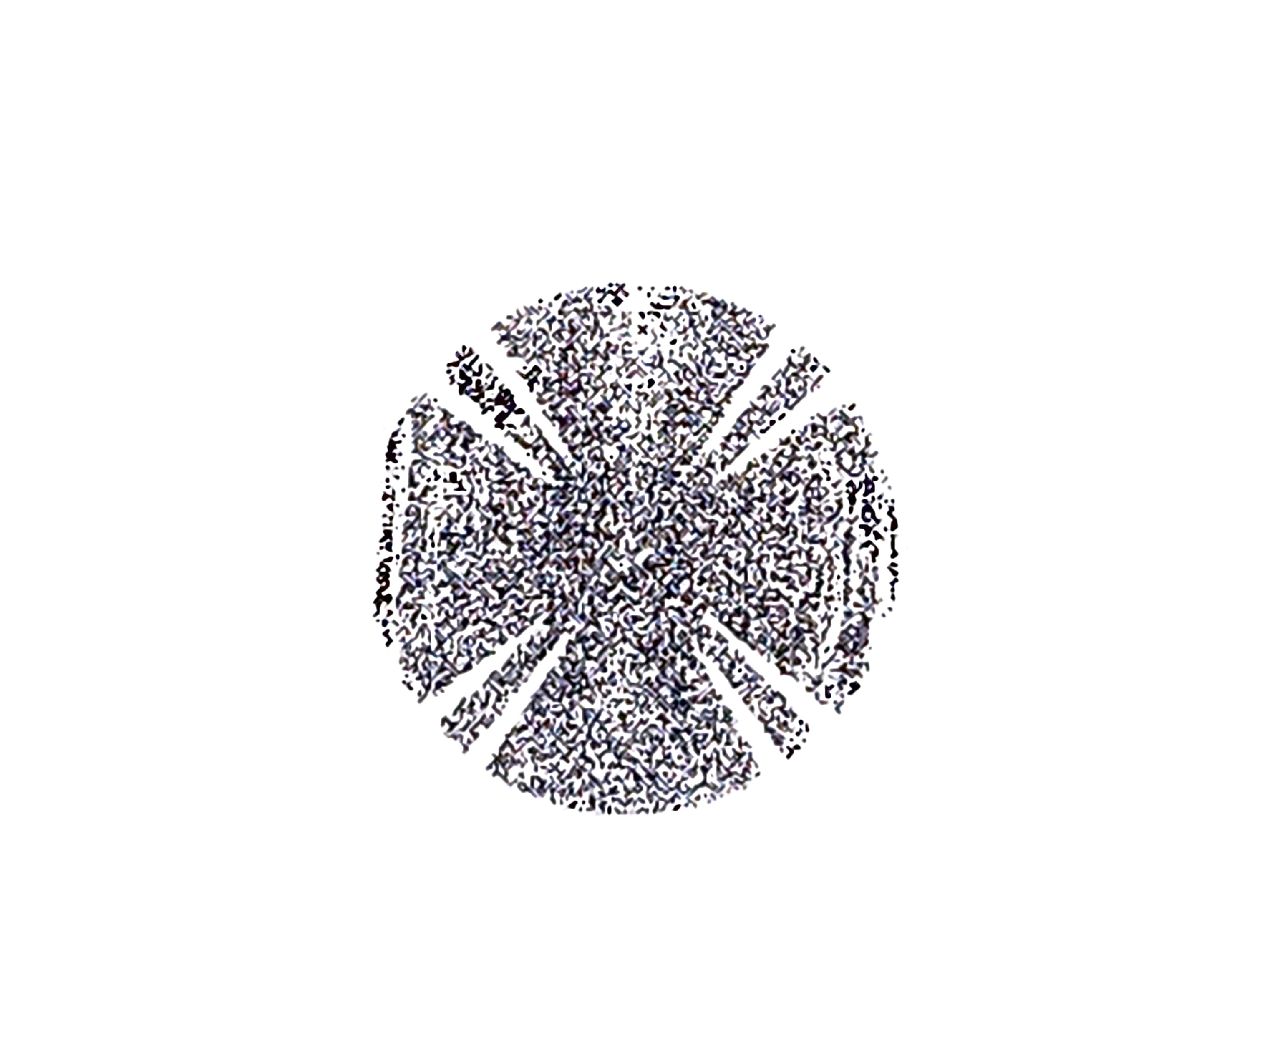
\includegraphics[width=.8\linewidth]{img/slam_1.pdf}
  \caption{全スキャンを同じ位置においた結果\cite{slam:nyumon}}
  \label{slam:scan}
  \end{center}
\end{figure}

\begin{figure}[h]
  \begin{center}
  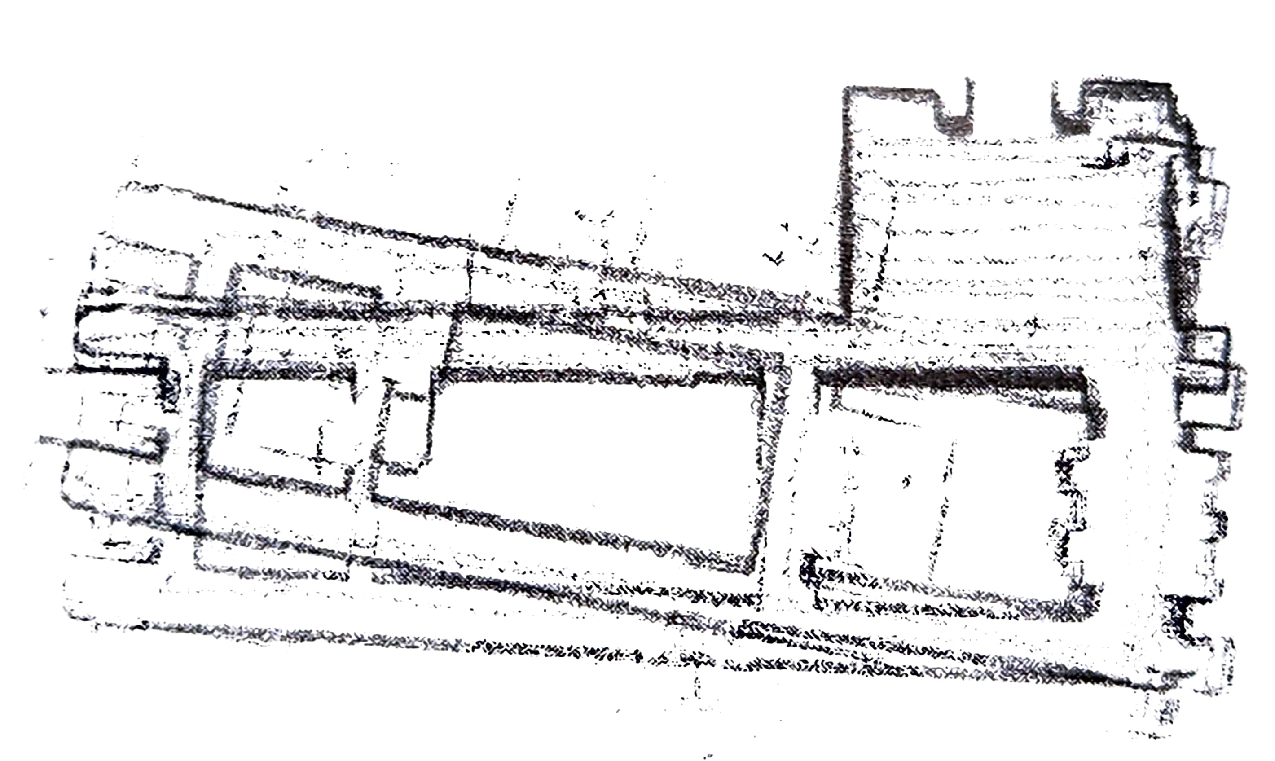
\includegraphics[width=.8\linewidth]{img/slam_2.pdf}
  \caption{オドメトリによる地図\cite{slam:nyumon}}
  \label{slam:odometry}
  \end{center}
\end{figure}

\begin{figure}[h]
  \begin{center}
  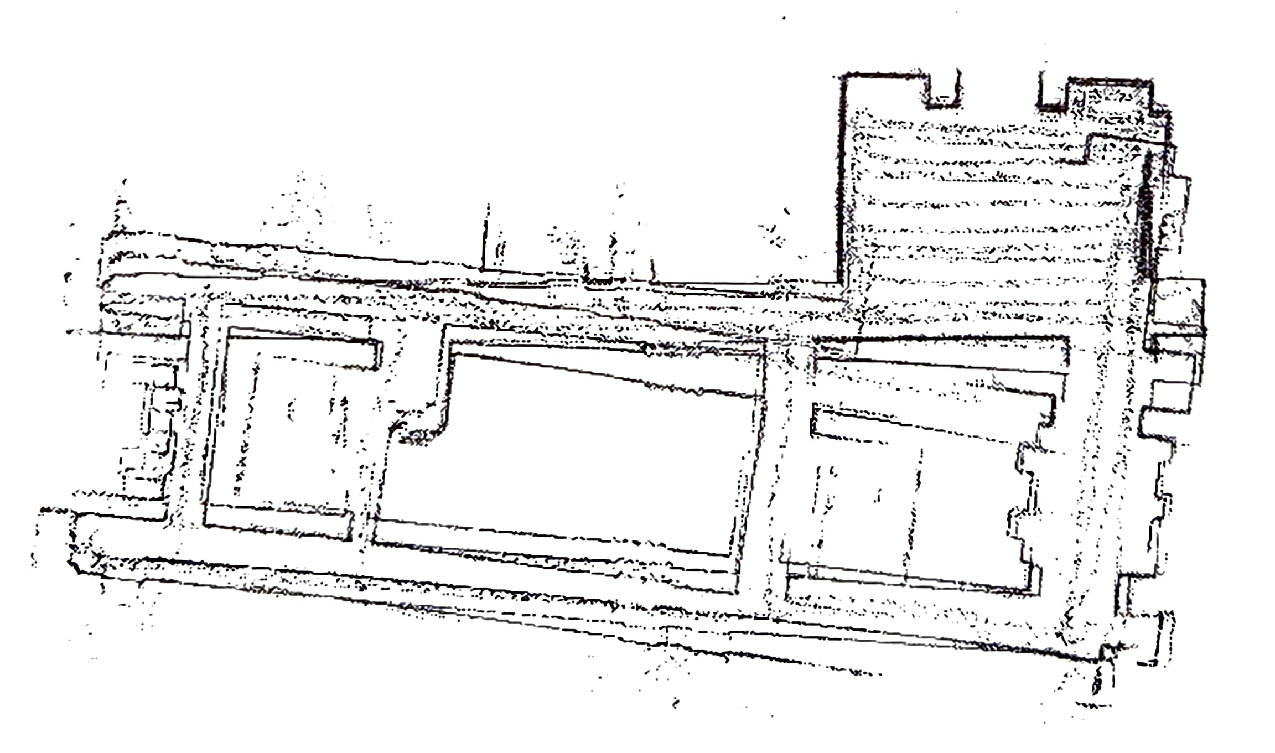
\includegraphics[width=.8\linewidth]{img/slam_3.pdf}
  \caption{SLAMによる地図(ループ閉じ込みなし)\cite{slam:nyumon}}
  \label{slam:slam}
  \end{center}
\end{figure}

\begin{figure}[h]
  \begin{center}
  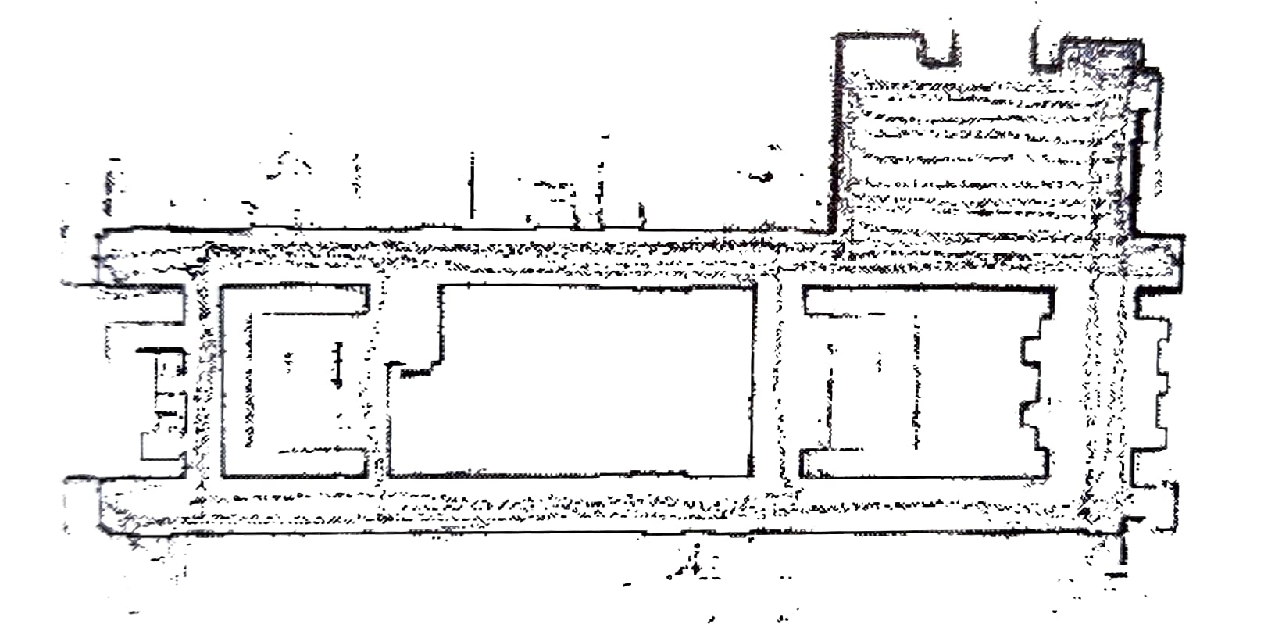
\includegraphics[width=.8\linewidth]{img/slam_4.pdf}
  \caption{SLAMによる地図(ループ閉じ込みあり)\cite{slam:nyumon}}
  \label{slam:slam_loop}
  \end{center}
\end{figure}

SLAMを用いることで、この歪みを減らすことができる。
SLAMには大きくレベルが2段階あり、ループ閉じ込みという技術を用いないレベルでは図\ref{slam:slam}のように局所的なぶれや歪みは小さくなるが、全体的な歪みは残る。
ループ閉じ込みを行うレベルでは図\ref{slam:slam_loop}のように全体形状の歪みも小さくなった地図をえることができる。
このようにSLAMは、ロボット位置と地図の推定を同時に行うことで、地図の精度を向上させる技術である。

\clearpage
\subsubsection{SLAMの実行形態}
SLAMを行う際にまず問題となるのは、センサデータ取得のための走行経路をどのように決めるかである。ロボットは地図を持っていないので、
どういう経路を通るのが安全で効率が良いか、あらかじめ知ることはできない。そこで、以下の2つの方法が考えられる。

\begin{enumerate}
  \item 人間がセンサデータの取得経路を与える\\
  対象環境をよく知っている人間がロボットにセンサデータ取得経路を与える。
  たとえば、人間がロボットを操縦してセンサデータを集める場合がこれにあたる。
  地図の生成は、操縦と同時に行う場合も、データ収集後にオフラインで行う場合もある。
  目的地への自律走行(ナビゲーション)を行う場合は、この方法で地図をつくることが多い。ナビゲーションでは、あらかじめ作成した地図の上で目的地への経路計画と自己位置推定を行うため、その場で地図を作る必要はないからである。
  ただし、ナビゲーションの最中に障害物や環境変化に対処するために、局所的な地図をその場で作って対処することは良くある。
  \item ロボットがセンサデータの取得経路を自律的に決める\\
  ロボットが自律走行してセンサデータを取得しつつ、リアルタイムに地図をつくる。
  その際、それまでに生成した地図と現在地周辺の局所的な地図を自律走行のために使う。ロボットは障害物を回避しながら走行し、次にどこに行くかを自分で決める必要があるため、SLAMだけでなく、探査、経路計画障害物回避なども含んだ総合的なシステムが必要になる。
  このようなシステムは、人間が操縦や遠隔操作をするのが難しい環境、あるいは、地図構築の知識をもったオペレータを用意できないアプリケーションなどで重要になる。理想はロボットが自律で地図を作ることであるが、実用においては目的に応じて使い分ければ良い。
\end{enumerate}

\subsubsection{SLAMの種類}
センサや地図には多くの種類があり、それに応じてSLAMの手法も変わる。
ここではSLAMの大きな分類軸として、2次元か3次元かを考える。
ロボットの位置(運動)と地図が、それぞれ2次元か3次元かで、原理的には4通りの分類ができる。
ここでは、ロボット位置/地図の次元によって、SLAMを2D/2D型、2D/3D型、3D/3D型に分けたものを表\ref{slam:table1}に示す。
(3D/2D型は事例が少ないため除外する。)

\begin{table}[h]
  \centering
  \caption{SLAMの種類}
  \scalebox{.9}{
  \begin{tabular}[t]{cccc}
    \toprule
    &ロボット位置&地図&センサ\\
    2D/2D型&2次元3自由度&2次元&2Dレーザスキャナ、オドメトリ、ジャイロ\\
    2D/3D型&2次元3自由度&3次元&2D/3Dレーザスキャナ、カメラ、オドメトリ、ジャイロ\\
    3D/3D型&3次元6自由度&3次元&3Dレーザスキャナ、カメラ、IMU\\
    \bottomrule
    \label{slam:table1}
  \end{tabular}}
\end{table}

これらのどの型を選ぶかは、ロボットの種類、タスク、コスト等によって変わる。
一般に2D/2D型、2D/3D型、3D/3D型の順に機能が高いと言えるが、コストもかかる機能的には3D/3D型が最も望ましいが、処理量が多いため、多くの場合、高性能コンピュータが必要になる。
ただし、最近は、地図の規模が小さければ、携帯端末レベルのコンピュータでも、3D/3D型SLAMが可能になっている。
移動機能を持ったロボットには、車輪型ロボット、クローラー型ロボット、脚型ロボット、ヒューマノイド、飛行ロボット等がある。
例えば、ヒューマノイドや飛行ロボットのように3次元の運動をするロボットには、3D/3D型が必要である。
車輪型ロボットは、地面や床面等の平面を走ることが多いので、2D/2D型が良く使われている。
ただし、障害物の検出には2D/3D型が有利であり、もし坂道や段差等を考慮するのであれば、車輪型ロボットでも3D/3D型SLAMが必要であると考えられる。

現在のSLAMシステムは、レーザスキャナを使ったものとカメラを使ったものに大別できる。
カメラはさらに、単眼カメラ、ステレオカメラ、距離画像カメラに分かれる。
2D-SLAMはレーザスキャナを用いるものが多く、また、古くから研究がおこなわれていたので、現在では実用レベルになっている。
代表的なものにGmapping\cite{slam:gmapping}やCartographer\cite{slam:cartographer}等がある。
3D-SLAMには、3Dレーザスキャナかカメラ、あるいはその両方が用いられる。

\subsection{SLAMの原理}
SLAMの原理を模式的に述べる。前提として、ロボットに搭載されたセンサのみを使う。
GPSなど、絶対位置が直接得られるセンサや装置は使わない。
簡単のため、ロボットにおけるセンサの設置個所は既知とし、両者の座標系は同一視する。
ロボット位置$\bm{x}$は方向も含めて$(x,y,\theta)^{\mathsf{T}}$ と表す。$x,y$ は、床面等の2次元座標系での位置(並進成分)、$\theta$ はロボットが向いている方向である。
なお、右肩の$\mathsf{T}$は、ベクトルの転置を表す。

\begin{figure}[h]
  \begin{center}
  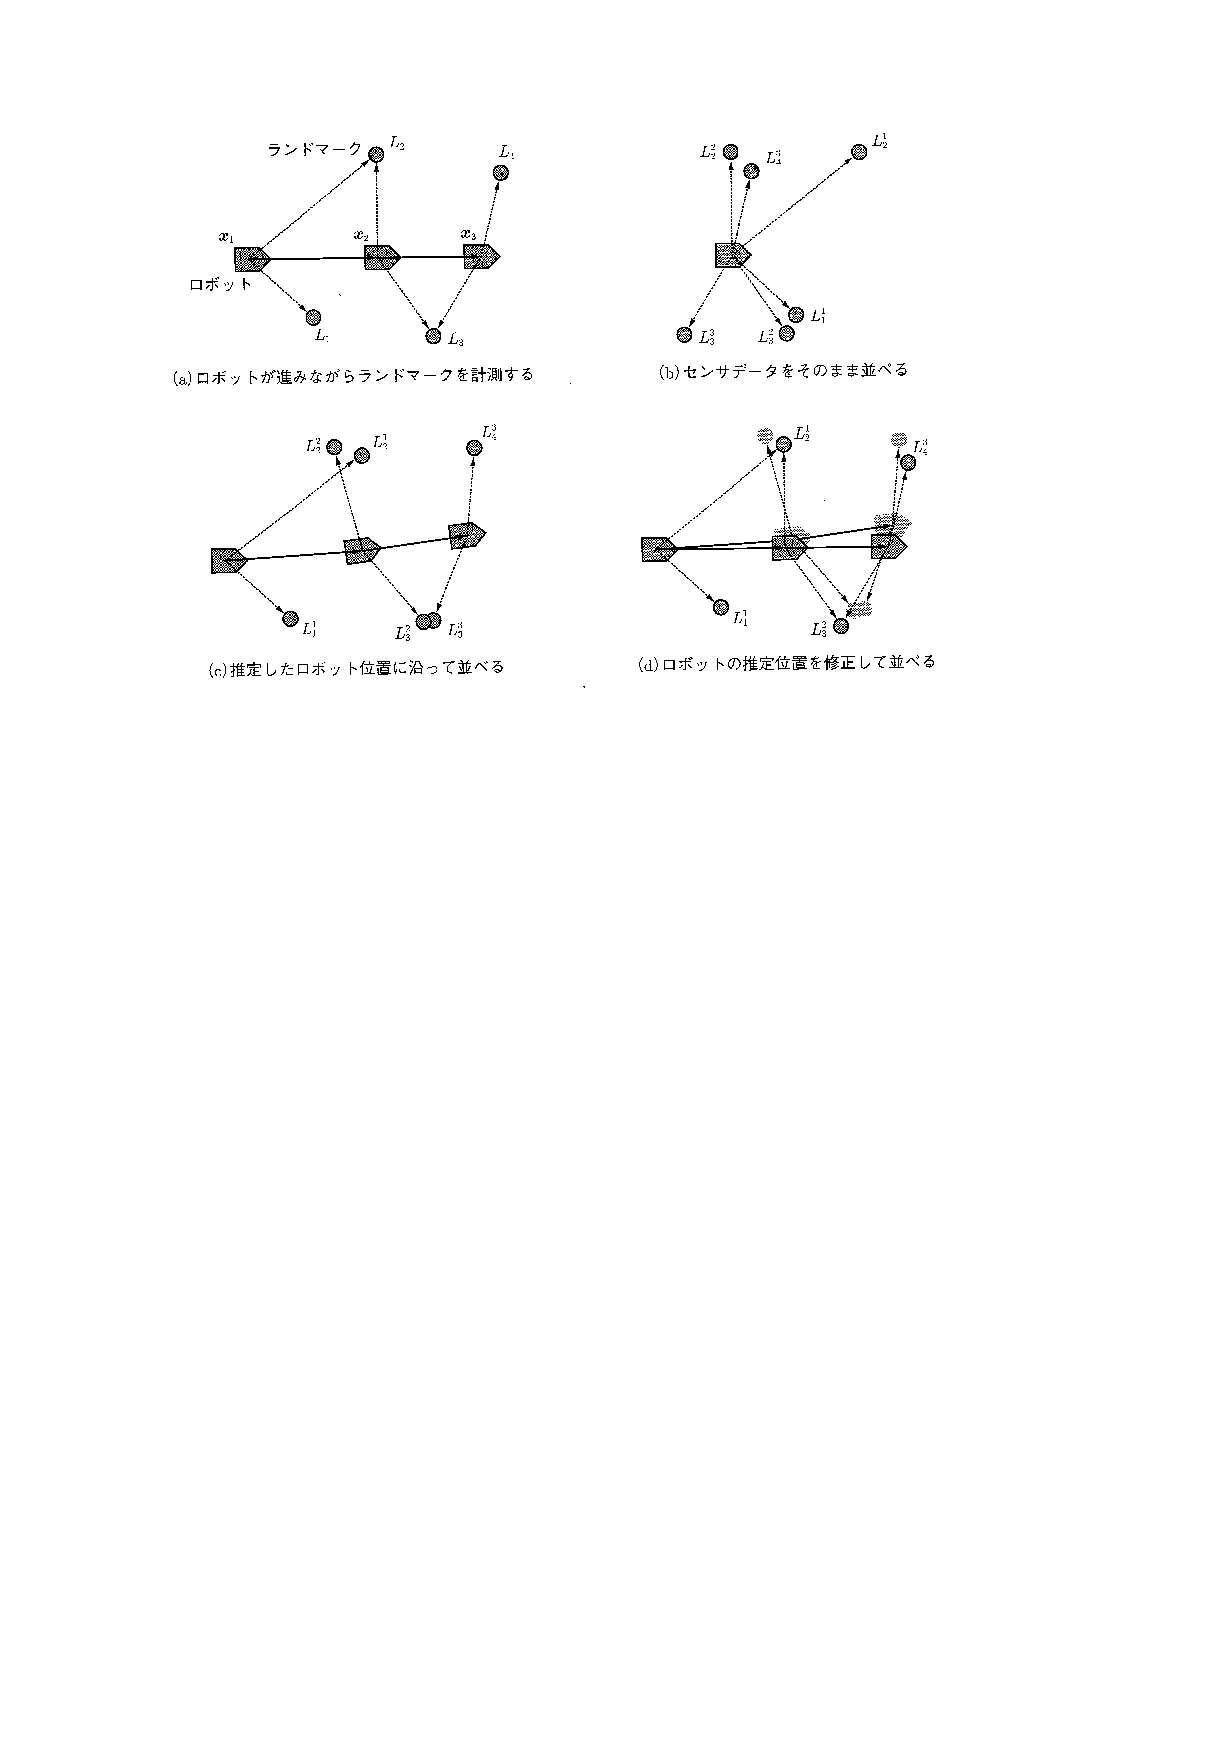
\includegraphics[width=\linewidth]{img/slam_5.pdf}
  \caption{ロボットで地図を作る様子\cite{slam:nyumon}}
  \label{slam:chizu1}
  \end{center}
\end{figure}

図\ref{slam:chizu1}にロボットで地図を作る様子を示す。地図はランドマークだけで構成されているとする。ランドマーク位置は点$\bm{q}$ で表す。
ランドマークに向きはない。この点では点がまばらにあるだけなので、障害物等の形状を表せず、地図としては不十分であるが、ロボットが位置を知るためには使える。
ここでも、ロボットは各ランドマークを区別できると仮定する。

\subsubsection{地図構築:ランドマーク位置の推定}
前述のように、ロボット位置が分かればランドマーク位置は計算できる。図\ref{slam:chizu2}\verb|~|図\ref{slam:suitei}に例を示す。この図では、
図\ref{slam:chizu1}のロボット位置$\bm{x_1}$ からランドマーク$\bm{q_2}$ を見る部分に注目している。$\bm{q_2}$ の地図座標系での位置を
$\bm{q_2}=(q_{2,x},q_{2,y})^{\mathsf{T}}$ また、センサの計測データ(センサ座標系の値)を$\bm{z_2} = (z_{2,x},z_{2,y})^{\mathsf{T}}$とする。
ここで、ロボット位置$\bm{x_1} = (x_1, y_1,\theta_1)^{\mathsf{T}}$ が分かれば、$\bm{q_2}$は式\eqref{slam:eq:q2}のように計算できる。

\begin{figure}[h]
  \begin{center}
  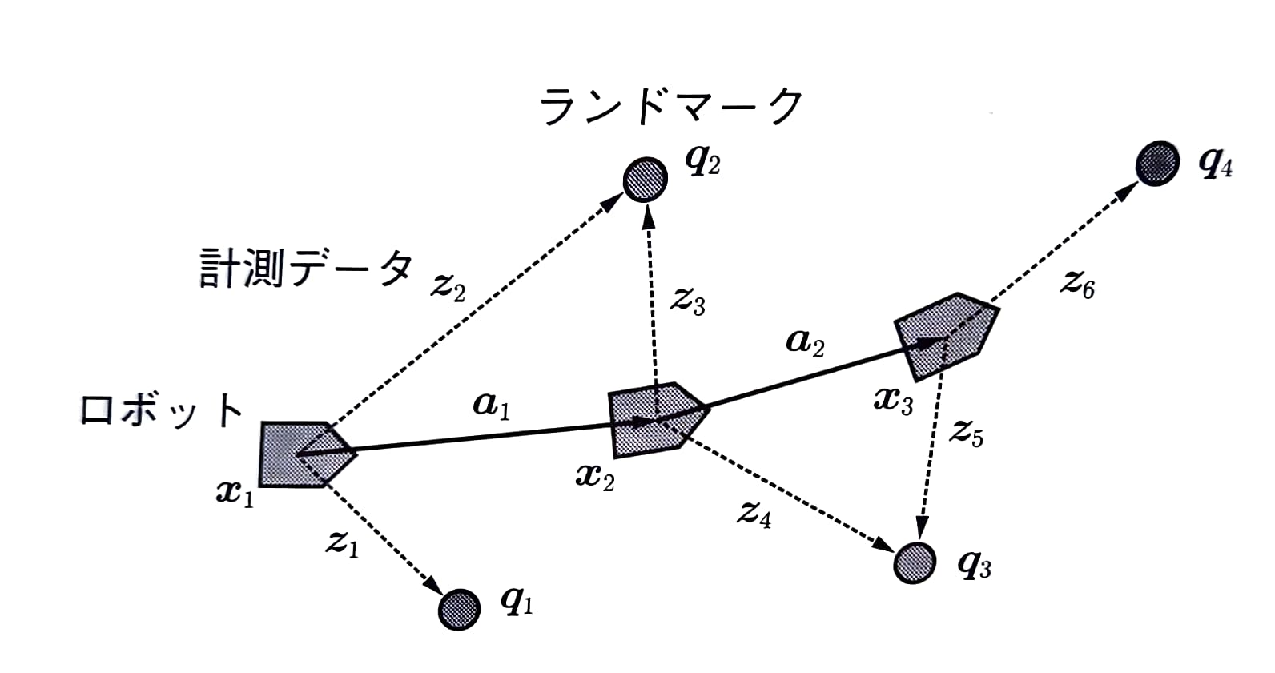
\includegraphics[width=\linewidth]{img/slam_6.pdf}
  \caption{ロボットとランドマークの位置推定\cite{slam:nyumon}}
  \label{slam:chizu2}
  \end{center}
\end{figure}

\begin{figure}[h]
  \begin{center}
  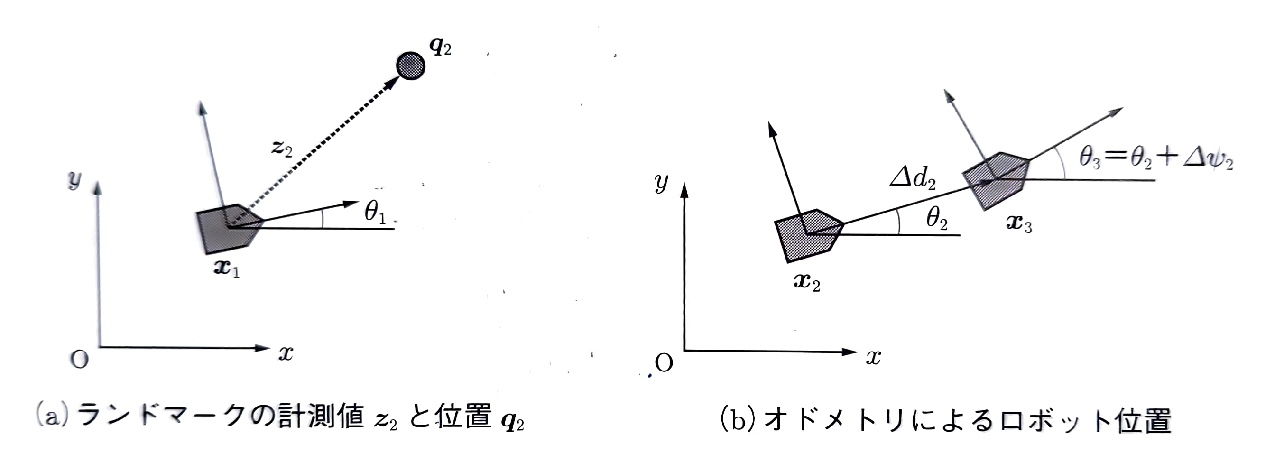
\includegraphics[width=\columnwidth]{img/slam_7.pdf}
  \caption{ランドマーク位置の推定とロボット位置の推定\cite{slam:nyumon}}
  \label{slam:suitei}
  \end{center}
\end{figure}

\clearpage

\begin{align}
  \begin{pmatrix}
    q_{2,x}\\
    q_{2,y}\\
  \end{pmatrix}
  =
  \begin{pmatrix}
    \cos\theta_1&-\sin\theta_1\\
    \sin\theta_1&\cos\theta_1\\
  \end{pmatrix}
  \begin{pmatrix}
    z_{2,x}\\
    z_{2,y}\\
  \end{pmatrix}
  +
  \begin{pmatrix}
    x_1\\
    y_1\\
  \end{pmatrix} \label{slam:eq:q2}
\end{align}

ここで、式を整理すると、
\begin{align}
  \bm{R_1} = 
  \begin{pmatrix}
    \cos\theta_1&-\sin\theta_1\\
    \sin\theta_1&\cos\theta_1\\
  \end{pmatrix},
  \bm{t_1} =
  \begin{pmatrix}
    x_1\\
    y_1\\
  \end{pmatrix}\label{slam:eq:q22}
\end{align}
なお、式\eqref{slam:eq:q22}は、式\eqref{slam:eq:q2f}のように表すことができる。
\begin{align}
  \bm{q_2} = \bm{R_1}\bm{z_2}+\bm{t_1} \label{slam:eq:q2f}
\end{align}

なお、センサがレーザスキャナの場合、センサ中心からランドマークまでの距離$d_2$と方向$\phi$を計測する。
すると、$z_2 = (d_2\cos\phi_2,d_2\sin\phi_2)^{\mathsf{T}}$となる。

\subsubsection{ロボット位置の推定}
ロボット位置を推定する有力な方法の1つにオドメトリ(Odometry)がある。オドメトリは、与えられた初期位置から微小変位を積分して現在位置を求める仕組みである。
例えば、車輪ロボットでは、車輪の回転数から移動量を求める「車輪オドメトリ」が良く用いられる。オドメトリによるロボット位置の計算方法はいくつかあるが、ここでは、
図\ref{slam:suitei}を例に、簡単な方法を紹介する。この図では、図\ref{slam:chizu2}のロボットが$\bm{x_2}$ から$\bm{x_3}$に移動する様子を表している。
オドメトリで得た移動量(ロボット座標系での並進と回転)を$\bm{a_2} = (\Delta d_2,0,\Delta\psi_2)^{\mathsf{T}}$とする。オドメトリで得る移動量は短時間の微小量なので、
瞬間的にはロボットは直進しているとみなし、$y$成分は0にする。すると、ロボット位置は$\bm{x_3}$は次の式\eqref{slam:eq:x3}のように計算できる。

\begin{align}
  \begin{pmatrix}
    x_3\\
    y_3\\
    \theta_3\\
  \end{pmatrix}
  =
  \begin{pmatrix}
    \cos\theta_2&-\sin\theta_2&0\\
    \sin\theta_2&\cos\theta_2&0\\
    0&0&1\\
  \end{pmatrix}
  \begin{pmatrix}
    \Delta d_2\\
    0\\
    \Delta\psi\\
  \end{pmatrix}
  +
  \begin{pmatrix}
    x_2\\
    y_2\\
    \theta_2\\
  \end{pmatrix} \label{slam:eq:x3}
\end{align}

なお、図\ref{slam:chizu2}の$\bm{a_2}$は、微小量である。この計算は、回転成分を含めた座標変換といえるため、compounding演算子$\oplus$で表すことがある。
compounding演算子を用いると、式\eqref{slam:eq:x3}は次のように表すことができる。

\begin{align}
  \bm{x_3} = \bm{x_2}\oplus\bm{a_2}
\end{align}

オドメトリで位置を求めるには、最初に初期位置$x_1$を与え、そこを起点として式\eqref{slam:eq:x3}によって微小な移動量を次々に加算していく。
そうすると、ロボットの位置を時間経過ごとに計算することができる。しかし、オドメトリを移動量を加算していく積分計算なので、移動量に含まれる誤差も加算される。
このため、ロボット位置の誤差が累積してどんどん増えていくという問題がある。そのため、図\ref{slam:odometry}に示すように、オドメトリによる推定位置は走行するにつれてずれていく。
人間に例えると、目をつぶって歩数で距離を推測するようなものであり、歩いているうちに位置がずれる。

\subsubsection{ロボット位置とランドマーク位置の同時推定}
オドメトリには「走行するにつれて誤差が累積する」という問題がある。そのため、図\ref{slam:chizu1}のロボット位置のずれは、これを推定したものである。
この累積誤差を減らすには、センサデータを地図に登録されたランドマークと照合して、ロボット位置を修正する方法が有効的である。目をつぶって歩きながら、時々薄目を開けてランドマークを見て、
自分がどこにいるか確認するようなものである。この時重要なのは、同じランドマークを複数回計測することである。例えば、計測データ$\bm{z_3}$からも、式\eqref{slam:eq:z3}ロボット位置$\bm{x_2}$に関する計算式が得られる。
\begin{align}
  \bm{q_2} = \bm{R_2z_3+t_2} \label{slam:eq:z3}
\end{align}
既に計測したランドマークからロボット位置を逆算して修正するために、式\eqref{slam:eq:q2f}によって$\bm{q_2}$が既知になったと考え、
その$\bm{q_2}$を使って、式\eqref{slam:eq:z3}を用いて$\bm{x_2}$を逆算すれば、ロボット位置を修正できる。ただし、この式だけでは、制約が足りず
逆算できないので、より多くの計算式を立式する。図\ref{slam:chizu2}において、オドメトリとランドマーク計測の計算式を全て立式すると、以下のような連立方程式となる。

\begin{align*}
  \bm{q_1} = \bm{R_1z_1+t_1}\\
  \bm{q_2} = \bm{R_1z_2+t_1}\\
  \bm{q_2} = \bm{R_2z_3+t_2}\\
  \bm{q_3} = \bm{R_2z_4+t_2}\\
  \bm{q_4} = \bm{R_3z_1+t_3}\\
  \bm{x_2} = \bm{x_1\oplus a_1}\\
  \bm{x_3} = \bm{x_2\oplus a_2}\\
\end{align*}

これらの式の変数は、ロボット位置$\bm{x_i}$とランドマーク位置$\bm{q_j}$である。ただし、地図がない時点でロボットの初期位置$\bm{x_1}$は適当な定数(多くの場合、地図座標系の原点)にする。
そのため、変数としてのロボット位置は2個になる。そうすると、ロボット位置は3次元、ランドマーク位置は2次元なので、これらの式の変数は全てで$3\times 2+2\times 4 = 14$個、式は、
$2\times 6+3\times 2=18$個となり、変数より式の方が多い連立方程式となる。変数より式の方が多い連立方程式には、多くの場合、厳密な解が存在しないので、最小二乗法を用いて解くのが一般的である。
ただし、これらの式は非線形関数である三角関数を含むので、非線形最小二乗問題となる。一般的に、センサデータには誤差があり、ロボット位置や地図の推定値にも誤差が波及する。連立方程式を最小二乗問題として解くことは、
推定値の誤差を減らすことにもなる。

\subsubsection{外界センサが一度に大量に得られる場合}
外界センサによる1回の計測で1回の計測で多くのランドマークデータを取得できれば、オドメトリ無しでもロボット位置を決められる。
図\ref{slam:sensor}を例として考える。レーザスキャナやカメラを用いる場合にこれが可能になる。

\begin{figure}[h]
  \begin{center}
  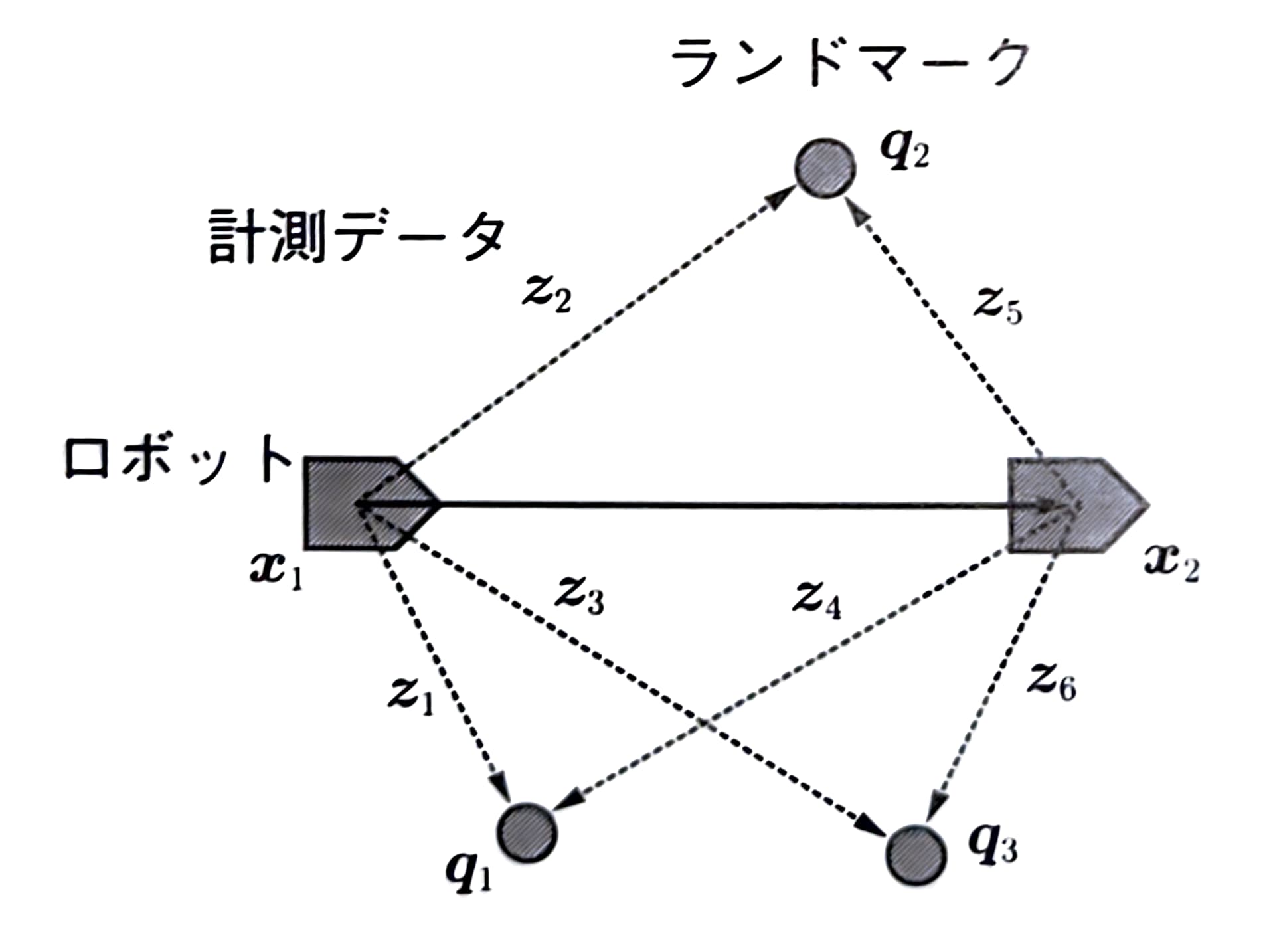
\includegraphics[width=.6\columnwidth]{img/slam_8.pdf}
  \caption{外界センサデータが一度に大量に得られる場合\cite{slam:nyumon}}
  \label{slam:sensor}
  \end{center}
\end{figure}

この図より得られる式は、式\eqref{slam:eq:sensor}に示す。
\begin{align}
  \begin{split}
    \bm{q_1} = \bm{R_1z_1+t_1}\\
    \bm{q_2} = \bm{R_1z_2+t_1}\\
    \bm{q_2} = \bm{R_1z_3+t_1}\\
    \bm{q_3} = \bm{R_2z_4+t_2}\\
    \bm{q_3} = \bm{R_3z_5+t_2}\\
    \bm{q_4} = \bm{R_3z_6+t_2} \label{slam:eq:sensor}
  \end{split}
\end{align}

ロボット位置は3次元、ランドマーク位置は2次元なので、これらの式の変数は全部で$3\times1+2\times3=9$個、式は
$2\times6 = 12$個となる。変数より式の方が多いので、前と同様に最小二乗法により解を求めることができる。この連立方程式にはオドメトリの制約が含まれていないが、
このように外界センサデータだけでロボット位置を求めることができる。上記の例はランドマークまでの距離と方向を計測できるレーザスキャナを用いた場合である。レーザスキャナのデータだけからロボット位置を求める方法には、例えば「スキャンマッチング」が挙げられる。

\subsection{要素技術}
ここではSLAMで必要となる要素技術について説明する。具体的にはこれまでの原理を実現する方法について述べる。

\subsubsection{不確実性の扱い}
センサデータには多くの誤差が含まれており、自己位置推定や地図構築に不確実性をもたらす。ここでは、偶然誤差の扱い方について述べる。偶然誤差はランダムに発生する確率で、
原因が特定できないため、確率的に扱う必要がある。前節の連立方程式には誤差が明示的に考慮されておらず、方程式自体はいわば誤差の無い理想的な状態を表しているが、現実ではそうはならない。
そこで、不確実性を扱うために、誤差を明示的に表す。式\eqref{slam:eq:q2f}を再喝する。
\begin{align*}
  \bm{q_2} = \bm{R_1z_2+t_1}
\end{align*}
これを次のように変形して、ロボット(センサ)座標系で見たランドマーク位置を考える。
\begin{align}
  \bm{z_2} = \bm{R_1^{-1}(q_2-t_1)}\eqdef \bm{h(x_1},\bm{q_2)}
\end{align}

ここで、$\eqdef$は定義を表す。$\bm{z_2}$は、実際の計測値、$\bm{h}$は、ロボット(センサ)座標系でのランドマーク位置を計算する関数である。
この式では等号を結んでいるが、実際は計測値$\bm{z_2}$に誤差があるため左の等式は成り立たない。そこで誤差を導入する。誤差は計測値と真値の差である。$\bm{x_1}$と$\bm{q_2}$は変数であるが、一旦それらを真値とみなすと、$\bm{z_2}$の誤差$\bm{v_2}$は次のようになる。
\begin{align}
  \bm{v_2} = \bm{z_2}-\bm{h(x_1},\bm{q_2)}
\end{align}

多くの誤差は正規分布に従うことで知られており、SLAMでも正規分布が最もよく使われる。そこで、ここでの誤差$v_2$も正規分布に従うと仮定することにする。
正規分布は平均と分散(多次元の場合は共分散行列)の2つのパラメータで定義できるので、$\bm{v_2}$も正規分布に従うと仮定する。正規分布は平均と分散(多次元の場合は共分散行列)の2つのパラメータで定義できるので、
$\bm{v_2}$の平均を$\bm{\mu_2}$、共分散行列を$\Sigma_2$とすると、$\bm{v_2}$は式\eqref{slam:eq:keisoku}の正規分布で表される。

\begin{align}
  p(\bm{v_2}) =\frac{1}{\sqrt{|2\pi\Sigma_2|}}\exp\biggl\{-\frac{1}{2}(\bm{v_2}-\bm{\mu_2})^{\rm{T}}\Sigma_2^{-1}(\bm{v_2-\mu_2})\biggr\}
\end{align}

\begin{align}
  p(\bm{v_2}) =\frac{1}{\sqrt{|2\pi\Sigma_2|}}\exp\biggl\{-\frac{1}{2}(\bm{z_2}-\bm{h}(\bm{x_1},\bm{q_2}))^{\rm{T}}\Sigma_2^{-1}(\bm{z_2}-\bm{h}(\bm{x_1},\bm{q_2}))\biggr\}\label{slam:eq:keisoku}
\end{align}

これを計測モデル(観測モデル)という。オドメトリの誤差も同様に式\eqref{slam:eq:x3}を例にすると、関数$\bm{g}$を使って、次のように表す。
\begin{align*}
  \bm{x_3} = \bm{x_2}\oplus \bm{a_2} \eqdef \bm{g}(\bm{x_2},\bm{a_2})
\end{align*}

これに、誤差$\bm{u_2}$を導入し、次のように表す。
\begin{align*}
  \bm{u_2} = \bm{x_3}-\bm{g}(\bm{x_2,a_2})
\end{align*}

上と同様に、誤差$\bm{u_2}$を導入して、式\eqref{slam:eq:undou}のように表す。
\begin{align}
  p(\bm{u_2}) = \frac{1}{\sqrt{|2\pi\Sigma_3|}}\exp\biggl\{-\frac{1}{2}(\bm{x_3}-\bm{g}(\bm{x_2},\bm{a_2}))^{\rm{T}}\Sigma_2^{-1}(\bm{x_3}-\bm{g}(\bm{x_2},\bm{a_2}))\biggr\} \label{slam:eq:undou}
\end{align}
と表す。これを運動モデルと呼ぶ。前の連立方程式の全誤差の確率密度$p$は、$u_i, v_j$の確率密度$p$を掛け合わせたものになる。

\begin{align}
  p = \prod_{i=1}^{2}p(\bm{u_i})\prod_{j=1}^{6}p(\bm{v_i})
\end{align}

この式はSLAMの構造を完全に表しており、この確率密度$p$を推定する問題は完全SLAM問題と呼ばれている。
この式は、最終的には、非線形最小二乗問題に帰着される。

\subsubsection{データ対応付け}
データ対応付け(data association)とは、「別々に計画されたセンサデータで、同じものを対応づけること」である。
SLAMでは、とくに、現在計測したセンサデータと、地図に登録されたランドマークの対応付けが重要になる。
「ロボットはランドマークを区別できる」という前提でSLAMの原理を説明した。
例えば、ICタグやビーコン等でID(識別子)が付いたランドマークであれば、IDをもとに一意に区別することが可能である。
このような装置を用いてロボットが場所や物体を認識する研究もなされており、目的・応用によっては非常に有効である。
一方SLAMでは、もともと存在する地形・風景・物体等を(IDのない)ランドマークとして用いることがよく行われている。
IDの無いランドマークを区別してデータ対応付けを行うのは、そう簡単ではない。
IDに変わる手がかりとして、ランドマーク位置と特徴量がよく使われる。

\begin{enumerate}
  \item 位置制約による対応づけ\\
  自己位置がある程度の精度で推定できるならば、その周辺の地図に登録されたランドマーク位置も予測できる。
  「自分は今地点Aにいるので、この方向にランドマークBが存在するはず」という具合である。そうすると、周辺のランドマーク位置を予想して、
  現在取得したセンサデータに最も近いものを対応づけるという方法が考え付く。非常によく用いられる。
  \item 特徴量による対応づけ\\
  センサデータとランドマークになんらかの特徴量を付加して、その特徴量によって両者の対応付けを行う方法である。特徴量はセンサによって多種多様で、
  レーザスキャンなら局所記述子やレーザの反射強度、カメラ画像ならば局所記述子や少領域の色・形状等がある。強力な特徴量ならば、それだけでかなりの対応づけができる。
  単純な特徴量では、それだけで対応づけるのは難しいが、候補の絞り込みに使うことができる。
\end{enumerate}

一般には、位置制約だけで対応付けを行うのは十分ではない。同じぐらいの位置に2つのランドマークがあった時に、どちらに対応づけるのが良いか判断するのが難しいからである。
逆に、特報量を用いる場合も、それだけで対応付けを完結するのは危険である。形状や外見が良く似たランドマークは区別が難しいからである。このため、特徴量を用いて対応候補を減らした上で
位置の探索範囲が狭く、しかも、一度に多くのセンサデータを計測できる場合は、位置制約だけで対応づけが上手くいく可能性が高くなる。
探索範囲が狭いために、対応付けの候補が少なく、しかも、同時に計測したデータ間の位置制約も使えるからである。「スキャンマッチング」という手法では、この性質を利用する。

\subsubsection{センサ融合}
前のように、大量データを一度に取得できる外界センサがあれば、基本的には、オドメトリ無しでSLAMを行うことが可能である。
しかし、実際には、そのような外界センサを用いても状況によっては大量データを得られないことがあり、センサデータに十分な情報が含まれていない場合もある。例えば、極端な場合、センサデータにランドマークが1つも含まれていない場合もある。
センサデータにランドマークが1つも含まれていなければ、ロボット位置は推定できない。この場合は、オドメトリを使うしか方法はない。さらにセンサデータは取れているが、情報が不足している場合等が考えられる。オドメトリを使わない場合、一度に得たセンサデータにランドマークが1個しか含まれていなければ、それだけではロボット位置を確定できない。前節でのSLAMの定式化では、オドメトリを用いていたので、ランドマークが1個でも、連立方程式の一部として、ロボット位置の推定に活かすことができた。しかし、オドメトリを使わない場合、センサデータにランドマークが1個しか含まれないとロボット位置は不定になってしまう。
例えば、式\eqref{slam:eq:q2}では、ロボット位置が変数3個に対して、方程式は2個しかないので、解は不定になる。
一般には、センサデータにランドマークが多く含まれているほど、安定して解が得られる。
ところが、センサデータにランドマークが多数含まれても、上手くいかない場合がある。
例えば、長い廊下にロボットがいる場合を考えてみる。
今、外界センサによって壁を計測してロボット位置を推定することを考える。
廊下の2つの壁は平行なので、その地図は計測点が2本の平行な直線上に並んだようになる。
同様に、センサデータも2本の平行な直線になる。壁に模様がないと仮定すると、この2本の直線を使ってロボット位置を一意に確定することはできない。
地図とセンサデータは、これらの直線に垂直な方向には位置が決まるが、平行な方向にはどこの位置でも合うからである。
このような状況を退化という。このように一度に大量のデータを計測できるセンサを用いたとしても、状況によっては情報が不足することがあり、ロボット位置を確定できなくなる。
このため、ロボットが安定して動作するためには、1つの外界センサだけでなく、オドメトリのような他のセンサを併用することが重要である。

\subsubsection{ループ閉じ込み}
SLAMにおいて重要な概念にループがある。図\ref{slam:loop_kiseki}にロボットの軌跡のループを示す。
ループとは周回路のことで、以前通った場所を再び通る経路である。SLAMによってランドマークを複数回計測してオドメトリによるロボット位置の累積誤差を減らした。これによって累積誤差は減るが、完全には消せない。
それは、ランドマーク計測にも誤差があるからである。ランドマーク位置が外部からあたえられたもの(既存地図など)であれば、誤差は累積しない。しかし、SLAMにおいては、ランドマーク位置も自分で推定したものなので、
ランドマーク位置に誤差が入り、そのランドマークを基準に自己位置すいていするとまた誤差が生じて、というように、誤差は累積していく。
SLAMでロボット位置の累積誤差をオドメトリ単体の場合よりも減らせるのは、その誤差の増加が、たいていはオドメトリ単体の場合より小さいからである。

\begin{figure}[h]
  \begin{center}
  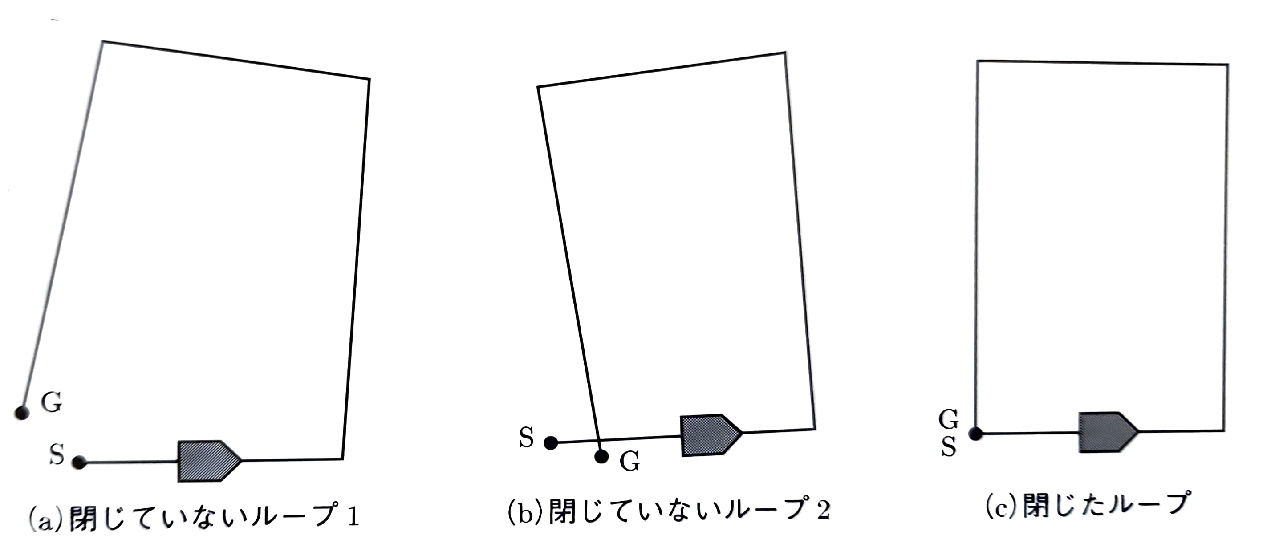
\includegraphics[width=.8\linewidth]{img/slam_9.pdf}
  \caption{ロボットの軌跡のループ\cite{slam:nyumon}}
  \label{slam:loop_kiseki}
  \end{center}
\end{figure}

このように、SLAMにも累積誤差があるので、ループは多くの場合、閉じない。図\ref{slam:loop_kiseki}に例を示す。
ロボットはS(スタート)から出発して1周し、Sと同じ位置にあるG(ゴール)に行くとする。この図で(a)は開いてしまった例、
(b)は重なってしまった例である。このように地図が歪んで実世界との違いが大きくなれば、ロボットが壁や障害物に衝突するかもしれない。
さらに困るのは、地図が歪んで実世界との違いが大きくなれば、ロボットが壁や障害物に衝突するかもしれない。さらに困るのは、地図が歪んで経路の接続関係が変わることである。
たとえば、経路がつながらなかったり、偽の交差点ができたりすると目的地までの経路を上手く見つけられなくなる。このため、ループを閉じることがSLAMの重要な処理になる。
これをループ閉じ込みという。(c)が、ループが閉じ状態である。ループ閉じ込みは次の手順で行う。

\begin{enumerate}
  \item ループ検出\\
  ロボットが同じ場所に戻ったことを検出する。ただし、まったく同じ座標に戻ることはめったになく、たいていは少しずれる。
  図\ref{slam:loop_detect}にループ閉じ込みの様子を示す。(a)は、ループがまだ閉じていない状態である。位置$\bm{x_k}$で、$\bm{x_1}$と同じランドマーク
  $\bm{q_1},\bm{q_2}$を計測したとする。$\bm{x_k}$は誤差によりずれているので、それにもとづいて配置したランドマーク位置$\bm{q_1^{\prime}},\bm{q_2^{\prime}}$もずれている。
  しかし、本来は同じランドマークなので、$\bm{q_1^{\prime}},\bm{q_2^{\prime}}$と、$\bm{q_1},\bm{q_2}$が同じになるようなロボットの位置
  $\hat{\bm{x_k}}$を求める。(a)ではループは閉じておらず、本来同じはずのランドマーク$\bm{q_1^{\prime}},\bm{q_2^{\prime}}$と、$\bm{q_1},\bm{q_2}$がずれている。(b)ではループ閉じ込み
  により正しいロボット位置$\hat{\bm{x_k}}$を見つけ、$\bm{q_1^{\prime}},\bm{q_2^{\prime}}$は、$\bm{q_1},\bm{q_2}$と一致している。
  
  \begin{figure}[h]
    \begin{center}
    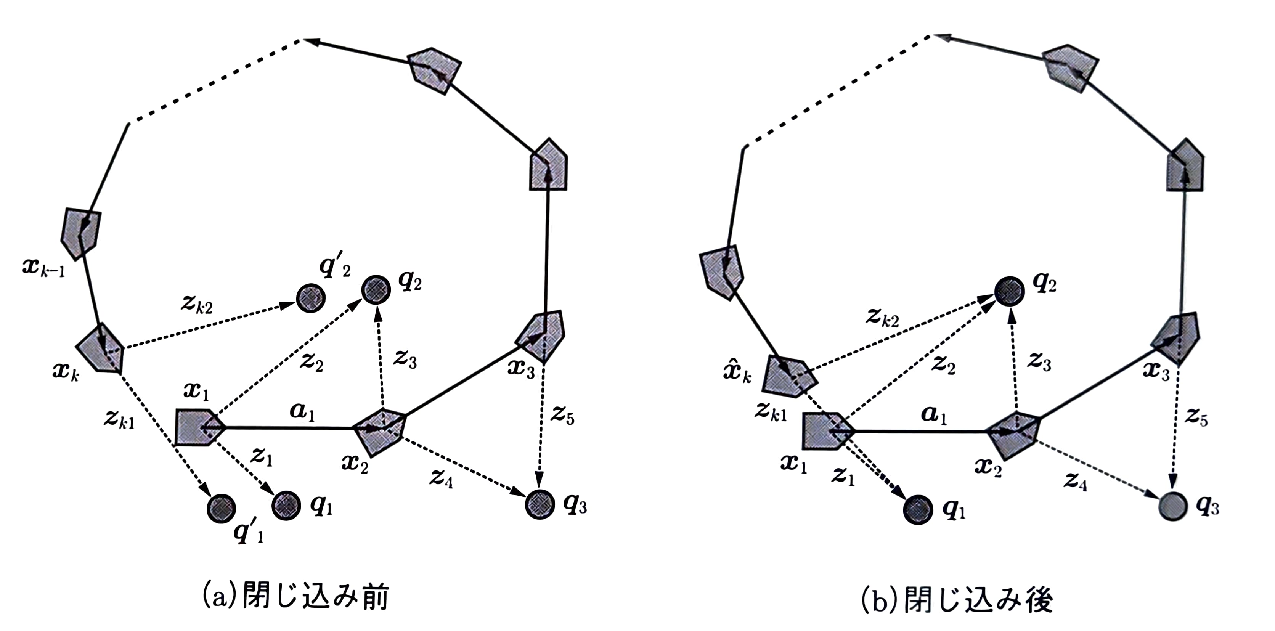
\includegraphics[width=.8\linewidth]{img/slam_10.pdf}
    \caption{ループ閉じ込みの様子\cite{slam:nyumon}}
    \label{slam:loop_detect}
    \end{center}
  \end{figure}
  \item ロボット軌跡と地図の修正\\
  図\ref{slam:loop_detect}で、ループを閉じると、$\bm{x_k}$は、$\hat{\bm{x_k}}$の位置に来るはずである。しかしそうすると、$\hat{\bm{x_k}}$と$\bm{x_{k-1}}$のずれが大きくなってしまうので、
  $\bm{x_{k-1}}$のずれが大きくなってしまうので、$\bm{x_{k-1}}$も修正する。こうして、逆向きにロボットの位置を修正していく。これに伴い、各ロボット位置で計測したランドマーク位置も修正する。
\end{enumerate}

この手順に従うと、軌跡を逆向きに修正していくことになるが、より効率的で精度が良いのは、連立方程式を一度に解くことである。ループ閉じ込みは、上で述べたSLAMの累積誤差を解消するのに有効である。ループが大きい程累積誤差は大きくなるので、それをループ閉じ込みで解消すれば、大きな誤差が一気に修正されたことになる。
以上の通り、ループ閉じ込みはSLAMの重要な要素技術であり、多くの研究が行われてきた背景にある。

\subsection{SLAMの処理形態:一括処理と逐次処理}
SLAMを連立方程式として考えると、センサデータを十分にそろえて、多くの方程式を立てた上で、一括で計算することになる。
前述の完全SLAM問題やループ閉じ込みは、基本的には一括処理である。
人間がロボットを操縦してセンサデータを集める場合は、このような一括処理で地図を作ることができる。
一方、ロボットが走行している最中に地図を作りたいことも良くある。
ロボットが自律的にセンサデータを集める場合は、センサデータを集めている最中にも地図が必要になる。
また、既存の地図を用いてナビゲーションを行っている場合でも、地図構築時とは環境が変化している可能性があるため、安全のために周囲の局所地図をリアルタイムで作り続けることが重要である。
このような場合は、連立方程式が全てそろうのを待たずに、それまでに収集された小数のセンサデータで作った部分的な連立方程式を解いて、逐次的に地図を構築していくことになる。
逐次的な地図構築は前節で述べたように、ロボット位置と地図を交互に求めていくことで行う。
すなわち、時刻$t-1$の地図に統合して、地図$t$の地図を求める。以上のように、SLAMの実行形態には、一括処理と逐次処理が考えられる。
それぞれの特徴を以下に示す。

\begin{enumerate}
  \item 一括処理の特徴
  \begin{itemize}
    \item センサデータが十分多く揃ってから行うため、リアルタイム処理に向かない。
    \item 多くのセンサデータを用いるので、処理時間は長いが、地図の精度は良い。
  \end{itemize}
  \item 逐次処理の特徴
  \begin{itemize}
    \item リアルタイムで逐次的に地図を構築する。このため、未知環境や変化する環境で行動する場合に有用である。
    \item 一部のセンサデータしか用いないので、処理時間は短いが、地図の精度は高くない。
  \end{itemize}
\end{enumerate}

なお、一括処理においても、必ずしも全センサデータがそろっている必要はない。十分多くのセンサデータがあれば、一括処理する意味がある。
実用上の一つの区切りは、ループを見つけるまでである。このように、両者は補完し合う性質を持つため、組み合わせて使うのが望ましい。

\subsection{Gmapping}
ここでは、SLAMの実証例であるGmappingについて述べる。
Gmappingのアルゴリズムは、Rao-Blackwellized Particle Filter (RBPF)によるGrid-Based SLAMである。
RBPFはベイズフィルタ系のパーティクルフィルタ(PF)の一種であり、SLAMにおいては、ロボット位置をPFで、地図を他の何らかのフィルタで推定するものと捉える。
ここでは、各パーティクルが現在のロボット位置だけでなく過去の走行軌跡も保持できる性質を利用している。
すなわち、パーティクルごとの走行軌跡に基づいて、各パーティクルで独立に地図を推定する。
パーティクルの数だけ、地図の仮説、ここでは占有格子地図が生成される。
占有格子地図の推定にはバイナリベイズフィルタによって、確率的に求められる。
Gmappingは、文献\cite{slam:gmapping}に示された格子ベースFast SLAMを実装したものである。以下にFastSLAMの流れを示す。

\begin{enumerate}
  \item 事前推定
  \begin{itemize}
    \item 動作モデルに従ってサンプリング
    \item 観測に従ってサンプルを更新(作成途中の地図情報を利用)
  \end{itemize}
  \item 観測更新1
  \begin{itemize}
    \item 重みを計算
  \end{itemize}
  \item 地図更新
  \begin{itemize}
    \item 地図を更新する(事前推定による状態値を利用)
  \end{itemize}
  \item 観測更新2
  \begin{itemize}
    \item 重みが最大となる粒子の状態値と地図を現時刻の推定値とする。
    \item 必要ならリサンプリングする。
  \end{itemize}
\end{enumerate}

なお、FastSLAMにも1.0と2.0が存在し、GmappingではFastSLAM2.0が実装されている。FastSLAMの流れについて、FastSLAM1.0から述べる。
前提として時刻$t$でロボットが移動している。今使える地図は、時刻$t-1$までに作成された中途半端なものである。この状態でロボットの位置と地図を更新することを考える。
図\ref{slam:zentei}に各々の時刻で作成された地図を示す。

\begin{figure}[h]
  \begin{center}
  \subfigure[時刻$t$までに作成された地図]{
  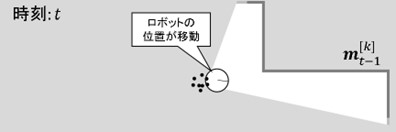
\includegraphics[width=.8\columnwidth]{img/slam_11.jpg}
  \label{slam:zentei1}
  }
  \subfigure[時刻$t-1$までに作成された地図]{
  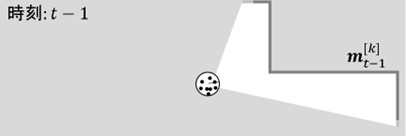
\includegraphics[width=.8\columnwidth]{img/slam_12.jpg}
  \label{slam:zentei2}
  }
  \caption{各時刻において作成された地図}
  \label{slam:zentei}
  \end{center}
\end{figure}

\subsubsection{事前推定}
今の時刻フレームでの地図を作成する前に、ロボットの動作モデル(制御指令に対する応答の予測体系:オドメトリ等)に従って、
今の時刻フレームにおける自己位置の候補点(位置と姿勢)に粒子を撒き、粒子の観測を行う。
動作モデルがホイールオドメトリならば、あらかじめホイールオドメトリに生じる誤差とその確率が明らかであれば、
それに従って点の撒き方が決定される。図\ref{slam:sample}にサンプルの撒き方の決定を示す。

\begin{figure}[h]
  \begin{center}
  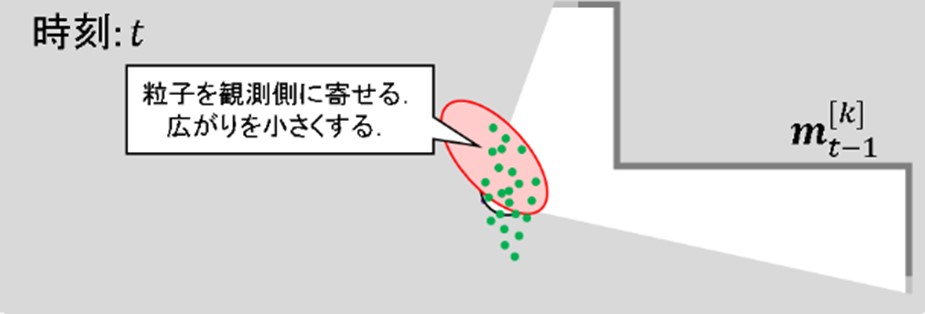
\includegraphics[width=.8\linewidth]{img/slam_13.jpg}
  \caption{サンプルの撒き方の決定}
  \label{slam:sample}
  \end{center}
\end{figure}

\subsubsection{観測更新1}
事前推定において撒いた各候補点から、既知の地図を観測した場合にどのように見えるかという予測と、
現在センサの実観測値を照合し、各候補点の尤度を計算し、各粒子の重みを更新する。図\ref{slam:sample_omomi}、\ref{slam:sample_yuudo}
に、尤度による重みの調整と事前推定を考慮した尤度の調整を示す。

\begin{figure}[h]
  \begin{center}
  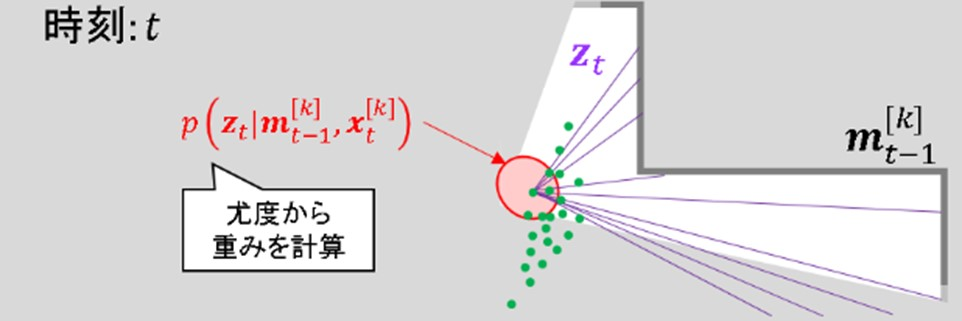
\includegraphics[width=.8\linewidth]{img/slam_14.jpg}
  \caption{尤度による重みの計算}
  \label{slam:sample_omomi}
  \end{center}
\end{figure}

\begin{figure}[h]
  \begin{center}
  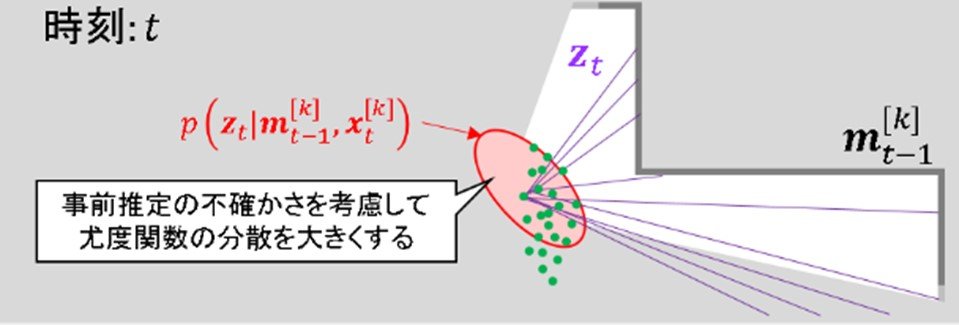
\includegraphics[width=.8\linewidth]{img/slam_15.jpg}
  \caption{事前推定を考慮した尤度の調整}
  \label{slam:sample_yuudo}
  \end{center}
\end{figure}

\subsubsection{地図更新}
各候補点それぞれを自己位置・姿勢であると仮定して、リサンプリングの前に地図を更新する。
図\ref{slam:sample_jikoichi}、\ref{slam:sample_chizu_koushin}に自己位置の仮定と、地図の更新を示す。

\begin{figure}[h]
  \begin{center}
  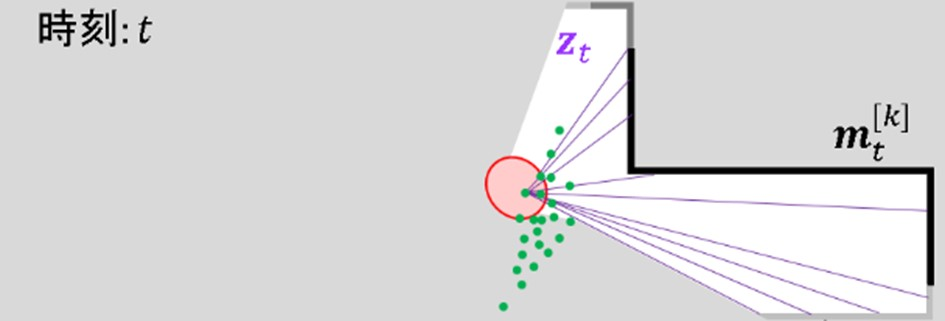
\includegraphics[width=.8\linewidth]{img/slam_16.jpg}
  \caption{自己位置の仮定}
  \label{slam:sample_jikoichi}
  \end{center}
\end{figure}

\begin{figure}[h]
  \begin{center}
  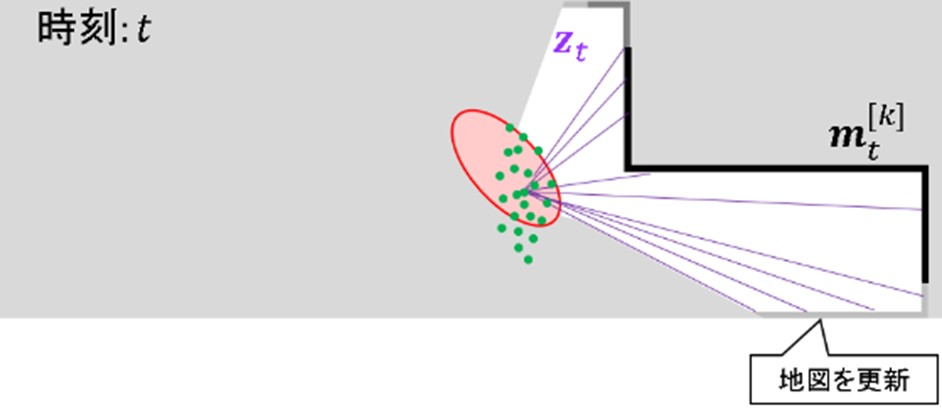
\includegraphics[width=.8\linewidth]{img/slam_17.jpg}
  \caption{地図の更新}
  \label{slam:sample_chizu_koushin}
  \end{center}
\end{figure}

\subsubsection{観測更新2}
地図を更新した後に、現時刻の推定値を確定する。最終的に、各候補点から「重みが最大」の粒子を選択し、
現在における自己位置推定結果として確定する。図\ref{slam:sample_suitei_kakutei}に自己位置推定結果の確定を示す。
また、図\ref{slam:sample_resampling}、\ref{slam:sample_tayou}に、粒子のサンプリングと粒子の多様性の考慮を示す。

\begin{figure}[h]
  \begin{center}
  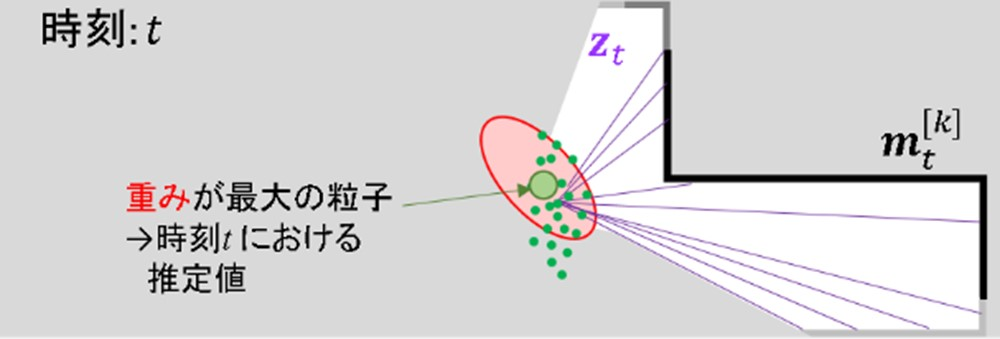
\includegraphics[width=.8\linewidth]{img/slam_18.jpg}
  \caption{自己位置推定結果の確定}
  \label{slam:sample_suitei_kakutei}
  \end{center}
\end{figure}

\begin{figure}[h]
  \begin{center}
  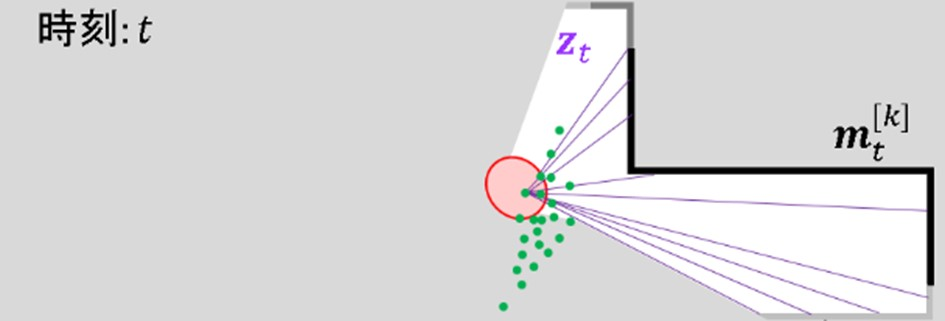
\includegraphics[width=.8\linewidth]{img/slam_19.jpg}
  \caption{粒子のリサンプリング}
  \label{slam:sample_resampling}
  \end{center}
\end{figure}

\begin{figure}[h]
  \begin{center}
  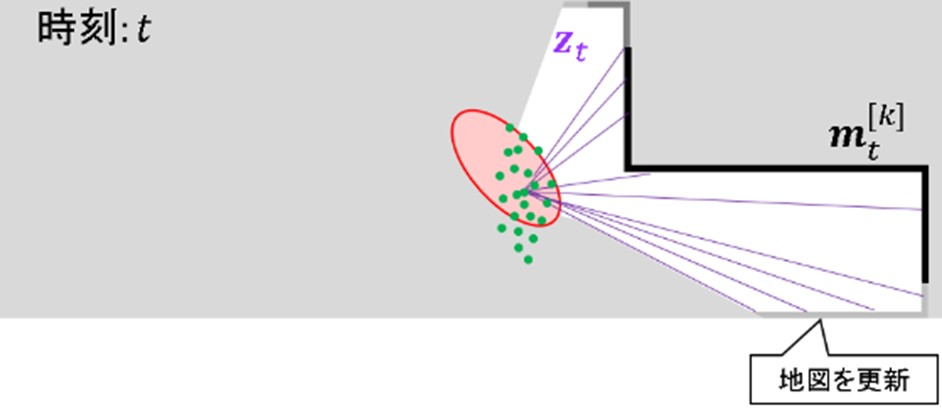
\includegraphics[width=.8\linewidth]{img/slam_20.jpg}
  \caption{粒子の多様性の考慮}
  \label{slam:sample_tayou}
  \end{center}
\end{figure}

\clearpage
\subsection{Hector SLAM}
ここでは、SLAMの実装例であるHector SLAMについて述べる。Hector SLAMは、スキャンマッチングで環境地図を構築している。
スキャンマッチングは、LiDARから刻々と得られる測定データを逐次重ね合わせていき、その際に生じる測定データの移動量からロボットの移動量を推定する手法である。
なお、スキャンマッチングに良く用いられる手法がICP(Iterative Closest Point)アルゴリズム\cite{slam:masuda}, \cite{slam:icp}である。Hector SLAMの場合も環境地図の構築に
ICPアルゴリズムの手法を取り入れている。Hector SLAMの場合、Gauss-Newton法で最適化を行い、最適されたものを式\eqref{slam:hector1}で剛体変換している。

\begin{align}
  \xi^{*} = \arg\min\sum_{i = 1}^{n} \left[1-\rm{M}(\rm{\bm{S}}_i(\bm{\xi}))\right]^2 \label{slam:hector1}
\end{align}

ここで、$\xi=(p_x,p_y,\psi)^{\rm{T}}$と、$\rm{\bm{S}}_i(\bm{\xi})$は、グローバル座標系におけるスキャンされた測定データ$i$の端点を表し、
ある連続したマップの座標$P_m$における占有値$\rm{M}(P_m)$は、サブ占有格子の精度を与えるためにバイリニアフィルタリングを用いて計算される。
式\ref{slam:eq:gauss}は、Gauss-Newton法を用いた$\Delta\xi$についての最小化させる式を表し、式\eqref{slam:eq:hesse}はそのヘッセ行列である。式\eqref{slam:eq:gauss}、\eqref{slam:eq:hesse}
は、占有値$\rm{M}(P_m)$すなわち、ある座標$P_m$におけるマップ勾配に依存する。

\begin{align}
  \Delta\xi = \rm{H}^{-1}\sum_{i = 1}^{n}\Biggl[\nabla M(S_i(\bm{\xi}))\frac{\partial\rm{S}_i(\bm{\xi})}{\partial\bm{\xi}}\Biggr]^{\rm{T}}[1-M(\rm{S}_i(\bm{\xi}))] \label{slam:eq:gauss}
\end{align}

\begin{align}
  \rm{H} = \Biggl[\nabla M(S_i(\bm{\xi}))\frac{\partial\rm{S}_i(\bm{\xi})}{\partial\xi}\Biggr]\Biggl[\nabla M(S_i(\bm{\xi}))\frac{\partial\bm{S}_i(\xi)}{\partial\bm{\xi}}\Biggr] \label{slam:eq:hesse}
\end{align}

\subsection{Cartographer}
Cartographerは、グリッドベースのスキャンマッチングによる逐次SLAMと一括処理のグラフベースSLAMの二種類で構成されている。
スキャンマッチングは、2Dの占有格子地図(Occupancy Grid Map)と、2D-LiDARから取得したスキャンデータを重ね合わせてロボットの自己位置を推定する処理である。
占有格子地図とは、環境を格子状に区切って、それぞれの格子に障害物が存在する確率(占有確率)を割り当てるものである。
例えば、黒い格子ほど占有確率が1に近く、白い格子ほど占有確率が0に近くなる。
また、LiDARは、センサから周囲の環境に向けてレーザ光を照射し、その反射光を受光素子で検知することで、センサから見た障害物までの距離と方向を取得する。
レーザ光が障害物に当たって跳ね返り、センサ中心まで戻ってくるまでの時間を計測することで、障害物までの距離を計算できる。
LiDARセンサが回転しながら、あらゆる方向に対レーザ光を照射するので、周囲の様々な障害物までの、距離と方向のペアが幾つも得られる。
LiDARセンサ1周分のデータをスキャンといい、周囲360度にある障害物(家具や壁など)の形状を反映した点群となる。スキャン同士、スキャンと地図、地図同士など、重ね合わせの対象にはいくつかの種類があるが、Scan-to-scan Matching, Scan-to-map Matching, Map-to-map Matchingなどと呼んで区別する。
ここでは、スキャンと占有格子地図の重ね合わせを扱うが、スキャン同士の場合と比べると誤差が小さいとされている。ICP(Iterative Closest Point)は、スキャン同士(Scan-to-scan)の場合と比べると誤差が小さいとされている。
ICP(Iterative Closest Point)とその派生、スキャン同士のマッチング手法、NDT(Normal Distributions Transform)は、スキャンと地図のマッチング手法に分類できる。
(NDTは占有格子地図ではなく、各格子が正規分布を表す格子地図を使う)。スキャンマッチングは、SLAMの核となる重要な処理である。
SLAMでは、ロボットの自己位置(ロボットが辿った軌跡)と、環境地図(占有格子地図)の2つを推定するが、これらの精度は、どのようなスキャンマッチングの手法を採用するかによって大きく左右される。
各手法には長所と短所があるので、計算量、メモリ消費、精度などの様々な観点から、最適なものを1つ選んで用いたり、あるいは複数の手法を組み合わせて用いたりすることが重要である。
グラフベースSLAMでは、明示的に再訪点を検出する。具体的には、現在地点の形状が過去の地図のある地点の形状と一致しているかを探索し、その地点が再訪点か判断する。
再訪点と現在値が一致するという拘束をかけ、ロボット軌跡の最適化を行う。

\subsubsection{分岐限定法によるスキャンマッチング}
2D-LiDAR SLAMの最先端であるCartographerでは、ループ検出に、分岐限定法(Branch-and-bound)ベースのスキャンマッチング手法を用いている。ループ検出(Loop Detection)とは、ロボットが以前訪れた場所に、再び戻ってきたことを検出するための処理で、
スキャンマッチングにより実現される。SLAMでは、直近のいくつかのLiDARスキャンをもとに占有格子地図を作成し、上記のような直近の観測データと最新の観測データとのマッチングだけを繰り返していくと、ロボットの位置現在位置には、
誤差が蓄積していき、本来の正しい位置から大きく外れる。ループ検出では、古い観測データと最新の観測データとのマッチングを行う。これより、ある場所を訪れてから、再びそこを訪れるまでの間に溜まった誤差を一気に解消し、
ロボットの現在位置を本来の正しい位置に戻すことができる。

ループ検出では、(以前その場所を訪れたときに取得した)古いスキャンを含む地図と、最新のスキャンとのマッチングを行う。
直近のスキャンとのマッチングによって、ロボットの現在位置は一応得られている。しかし、本来の位置からは大きくずれているので、ループ検出によって大幅に修正される。
つまり、初期値と最適解が離れているということである。ガウス・ニュートン法(Gauss-Newton法)やレーベンバーグ・マーカート法(Levenberg-Marquardt)、山登り法(Hill-Climing)のような逐次的なマッチング手法では、
初期値が最適解にある程度近いことが要求される。言い換えると、ロボットの現在位置が真値とかなり近く、誤差が少ない状態である(地図とスキャンとが既にある程度重なり合っている)ことが求められるが、ループ検出での前提とは異なる。
したがって、逐次的なマッチング手法は利用できず、初期値に依存しない頑健な手法が求められる。分岐限定法によるスキャンマッチングは、効率が良く、しかも頑健な手法であるため、ループ検出に利用できる。

\subsubsection{分岐限定法によるスキャンマッチングアルゴリズム}
最初に、アルゴリズムの入出力について述べる。入力とパラメータは次の通りである。

\begin{enumerate}
  \item 探索方向のサイズ:$(W_x,W_y,W_\theta)$、$(W_x,W_y)$は、単位\si{[m]}、$W_{\theta}$は\si{[rad]}
  \item $\theta$方向のステップサイズ:$\delta_\theta$\si{[rad]}
  \item ノードの高さ:$h_0$
  \item スキャンデータ:$\mathcal{S}=\{\rm{z_1},\ldots,\rm{z_N}\}={(r_1,\theta_1),\ldots, (r_N,\theta_N)}$
  \item 占有格子地図:$\mathcal{M}$:解像度$r$
  \item 探索領域の中心に対応する姿勢:$\xi_0 = [\xi_{0,x},\xi_{0,y},\xi_{0,\theta}]^{\rm{T}}$
\end{enumerate}
出力は次の通りである。
\begin{enumerate}
  \item 最大のスコア:$\bm{s}$
  \item スコアを最大化する姿勢:$\xi^{*}$
\end{enumerate}
アルゴリズムは以下のようにまとめられる。
\begin{enumerate}
  \item 探索領域サイズ(半径)$w_x,w_y,w_\theta$を計算し、探索領域$\overline{\mathcal{W}}$と$\mathcal{W}$を定める。\\
  $w_x = \left\lceil \frac{W_x}{r}\right\rceil, w_y = \left\lceil \frac{W_y}{r} \right\rceil, w_{\theta} = \left\lceil \frac{W_{\theta}}{\delta_{\theta}}\right\rceil$\\
  $\overline{\mathcal{W}} = \{0,\ldots,2w_x\}\times\{0,\ldots,2w_y\}\times\{0,\ldots,2w_{\theta}\}$\\
  $\mathcal{W} = \bigl\{\xi_0+[r(-w_x+j_y),r(-w_y+j_y),\delta_{\theta}(-w_{\theta+j_{\theta}})]^{\rm{T}}|(j_x,j_y,j_{\theta})\in\overline{\mathcal{W}}\bigr\}$
  \item 与えられた地図$\mathcal{M}$を基に、$h_0$個の地図$\mathcal{M}_{\rm{precomp}}^1,\ldots,\mathcal{M}_{\rm{precomp}}^{h_0}$を計算する。
  \begin{align*}
    \mathcal{M}_{\rm{precomp}}^1(i,j) = \max_{\substack{i\leq i^{\prime} < i+2^h\\j\leq j^{\prime}<j+2^h}} \mathcal{M}(i^{\prime},j^{\prime})  
  \end{align*}
  \item 空のスタック(あるいは優先度付きキュー)$\mathcal{C}$を$\mathcal{C}_0$で初期化する。$\mathcal{C}_0$はノードの集合であり、次のように定義される。\\
  $\overline{\mathcal{W}}_{0,x}=\bigl\{2^{h_0}j_x|j_x\in\mathbb{Z},0\leq 2^{h_0}j_x\leq 2w_x\bigr\}$\\
  $\overline{\mathcal{W}}_{0,y}=\bigl\{2^{h_0}j_y|j_y\in\mathbb{Z},0\leq 2^{h_0}j_y\leq 2w_y\bigr\}$\\
  $\overline{\mathcal{W}}_{0,\theta}=\bigl\{j_{\theta}|j_{\theta}\in\mathbb{Z},0\leq j_{\theta}\leq 2w_{\theta}\bigr\}$\\
  $\mathcal{C}_0 = \overline{\mathcal{W}}_{0,x}\times\overline{\mathcal{W}}_{0,y}\times\mathcal{W}_{0,\theta}\times\{h_0\}$\\
  各ノード$c=(2^{h_0}j_x,2^{h_0}j_y,j_{\theta},h_0)\in\mathcal{C}_0$について、$\mathcal{M}^{h_0}_{\rm{precomp}}$を使って、スコアの上界$\overline{s}(c)$が最も高いノードが、$\mathcal{C}$の先頭に来るように、$\mathcal{C}_0$に含まれる
  全ノードを$\mathcal{C}$に追加していく(上界も一緒に追加)。各$j_{\theta}$について、$I_{i,x}^0,I_{i,y}^0$は一度だけ計算すれば良い。\\
  \begin{align*}
    \overline{s}(c)=\sum_{i = 1}^{N}\mathcal{M}^{h_0}_{\rm{precomp}}(I_{i,x}^0+2^{h_0}j_x,I_{i,y}^{0}+2^{h_0}j_y)
  \end{align*}
  \begin{align*}
    I_{i,x}^0=\left\lfloor \frac{\xi_{0,x}+r_i\cos(\xi_{0,\theta}+\delta_{\theta}(-w_{\theta}+j_{\theta})+\theta_i)}{r} \right\rfloor - w_x
  \end{align*}
  \begin{align*}
    I_{i,y}^0=\left\lfloor \frac{\xi_{0,y}+r_i\sin(\xi_{0,\theta}+\delta_{\theta}(-w_{\theta}+j_{\theta})+\theta_i)}{r} \right\rfloor - w_y
  \end{align*}
  \item 最大のスコア$\bm{s}^{*}$を$-\infty$で、また最適解$(j_x^{*},j_y^{*},j_{\theta}^{*})\in\overline{\mathcal{M}}$を(0,0,0)で初期化する。
  \item キュー$\mathcal{C}$が空になるまで、以下を繰り返す。
  \begin{enumerate}
    \item $\mathcal{C}$の先頭から、ノード$c=(c_x,c_y,c_{\theta},h)$と上界$\overline{s}(c)$を取り出す。
    \item 枝刈り:上界$\overline{s}(c)$が、現在の最大値$\bm{s}^{*}$以下であれば、ノード$c$と、その子ノードの探索は不要であるから、\\
    上に戻って次のノードを試す。
    \item ノード$c$の高さが$h=0$、言い換えると葉ノードである場合は、現在の最大スコア$\bm{s}^*$を$\overline{s}(c)$、また最適解
    $(j_x^{*},j_y^{*},j_{\theta}^{*})$を$(c_x,c_y,c_{\theta})$で更新し、上に戻る。
    \item 分岐:ノードが葉ノードでなければ、4つの子ノード$c_1,c_2,c_3,c_4$に分割する。\\
    \begin{align*}
      c_1 = (c_x,c_y,c_{\theta},h-1)
    \end{align*}
    \begin{align*}
      c_2 = (c_x+2^{h-1},c_y,c_{\theta},h-1)
    \end{align*}
    \begin{align*}
      c_3 = (c_x,c_y+2^{h-1},c_{\theta},h-1)
    \end{align*}
    \begin{align*}
      c_4 = (c_x+2^{h-1},c_y+2^{h-1},c_{\theta},h-1)
    \end{align*}
  \end{enumerate}
  \item 各ノード$c_i$について上界$\overline{s}(c_i)$を計算する。以下は$c_3$の場合の計算式である。
  \begin{align*}
    \overline{s}(c_3) = \sum_{i=1}^{N}\mathcal{M}_{\rm{precomp}}^{h-1}(I_{i,x}^{0}+c_x+2^{h-1},I_{i,y}^{0}+c_y+2^{h-1})  
  \end{align*}
  \begin{align*}
    I_{i,x}^0 = \left\lfloor \frac{\xi_{0,x}+r_i\cos(\xi_{0,\theta}+\delta_{\theta}(-w_{\theta}+c_{\theta})+\theta_i)}{r}\right\rfloor -w_x
  \end{align*}
  \begin{align*}
    I_{i,y}^0 = \left\lfloor \frac{\xi_{0,y}+r_i\sin(\xi_{0,\theta}+\delta_{\theta}(-w_{\theta}+c_{\theta})+\theta_i)}{r}\right\rfloor -w_y
  \end{align*}
  \\
  上界の最も大きな子ノードが先頭に来るように、4つの子ノードを$\mathcal{C}$に追加していく(上界も一緒に追加)。
  \item 上記の手続きによって最適解$(j_x^{*},j_y^{*},j_{\theta}^{*})\in\overline{W}$が得られたので、最適な姿勢$\xi^{*}$を次のように計算する。\\
  \begin{align*}
    \xi^{*} = \bigl[\xi_{0,x}+r(-w_x+j_x^{*}),\xi_{0,y}+r(-w_y+j_y^{*}),\xi_{0,\theta}+\xi_{\theta}(-w_{\theta}+j_{\theta}^{*})\bigr]^{\mathsf{T}}
  \end{align*}
  \item 最大のスコア$\bm{s}^{*}$と、最適な姿勢$\xi^{*}$を返す。
\end{enumerate}

\subsection{SLAMによる環境地図の評価}
ここでは、LiDARを用いたSLAMによって生成された環境地図の評価に関する研究について述べる。

\subsubsection{Hector SLAMおよびGmappingの性能分析}
文献\cite{slam:comp1}によると、モバイルロボットのナビゲーションを目的としたHector SLAMおよびGMappingアルゴリズムの性能分析が行われている。
研究結果によると、Hector SLAMアルゴリズムの性能がGMappingよりも優れていることが示されている。
ここでは、2Dレーザスキャンデータと、Hector SLAMとGMappingアルゴリズムを使用して、2次元の占有格子地図を生成した。
生成されたマップの精度を評価するために、マップ長をRVizの測定ツールで測定を行っている。
測定の結果Hector SLAMアルゴリズムは、オドメトリを使用せずに地図を生成し、平均誤差が7.86 cmであった。
一方、GMappingアルゴリズムはオドメトリデータとスキャンデータを組み合わせて使用し、平均誤差が10.86 cmであることが示されている。
したがって、Hector SLAMアルゴリズムは、精度の面でGMappingアルゴリズムよりも優れていると結論付けられている。
文献での評価に用いられたハードウェア構成を以下に示す。
\begin{enumerate}
  \item Raspberry Pi:スキャンデータの処理、地図作成、通信、Arduinoとの通信(速度データ)
  \item Arduino:Raspberry Piとの通信、DCモータの制御、ロータリーエンコーダによるオドメトリの取得
  \item LiDAR:RPLiDAR-A1
\end{enumerate}

ここで、この文献上では、環境地図生成のためのオドメトリ情報としてロータリーエンコーダを用いており、
LiDARのみでのSLAMの性能の比較は行われていない。Hector SLAMアルゴリズムは、環境地図生成のためのオドメトリが必要でないアルゴリズムである。
一方Gmappingは、オドメトリが必須である。しかし、比較を行うならば、GmappingをLiDARのみで動作させるべきである。
また、これらのSLAMのパッケージでは、パラメータの値により処理のパフォーマンスが変わる可能性があるため、それぞれのSLAMのパッケージに応じたパラメータの与え方を調整する必要がある。

\subsubsection{Grand truthデータとLiDARを用いた2D SLAMアルゴリズムの地図比較}
文献\cite{slam:grandtruth}によると、ROSのGmapping、Cartographer、Hector SLAMの3つのSLAMアルゴリズムによって、作成された地図と、レーザトラッカーによって示された
Grand truth(AIモデルの出力の教師あり学習で使われる正解データ)の比較が行われた。地図は、静的な屋内環境で行われ、Grand truthモデルは非常に精度が高いものが使用されている。
地図空間上の点座標をマイクロメートル精度で計測する高精度レーザートラッカーFAROによって構築されたGrand truthを用いて、SLAM地図の品質を評価する手法が提案された。実験は、移動ロボットの動作について、
以下の異なる条件で行われた。(1)滑らかなターンで素早く、(2)急旋回を伴う高速移動、(3)スムーズな旋回を伴う低速移動。(4)スムーズなターンでゆっくり、ただしループは閉じない。結果として、
おおよそほとんどの条件でCartographerが、レーザートラッカーが提示するGrand truthに対して、最小の誤差で地図を構築することが明らかになった。このアルゴリズムは、様々なタイプの移動ロボットの動きに対して、十分に強固であるとした。
Gmappingの地図は、Cartographerの地図の品質と同等であった。その理由はGmappingは、2D地図構築において、ループ閉じ込みがなくても、自己位置の地図の補正にオドメトリを使用しているからである。
これは、Cartographerについても同様である。Hector SLAMの最先端であるCartographerではLiDARデータのみを使用し、ループ閉じ込みを行わない。そのため、Hector SLAMの結果は精度が悪いとしている。
このようにCartographerが、LiDARを移動ロボットに搭載し、2Dの地図を生成するのに最適なアルゴリズムであると結論づけた。文献\cite{slam:grandtruth}の実験で使用された差動駆動移動ロボットプラットフォームについて示す。

\begin{enumerate}
  \item オンボードコンピュータ Jetson TX1
  \item バンパー
  \item ソナー
  \item Troyka IMU モジュール
  \item Hokuyo URG-04LX-UG01 二次元LiDAR
  \item Velodyne WLP-16 三次元LiDAR
  \item 車輪のオドメトリを計算するためのロータリーエンコーダ
  \item ROS Kinetic Ubuntu 16.04
\end{enumerate}

ここでも文献上では、ロータリーエンコーダやIMU等の内界センサによるオドメトリによって自己位置と地図の補正を行っていて、LiDARのみでのSLAMの地図精度の評価は行われていない。また、先に述べた文献と比較すると、
Hecor SLAMよりも、Gmappingのアルゴリズムの方が優れているとした、異なる結果が得られている。これらの違いは、RVizによる手動測定ではなく、レーザートラッカーによるGrand truthデータを用いている点、地図生成GPUを搭載した
高性能なコンピュータを用いている点である。前述のように、SLAMアルゴリズムや、各アルゴリズムで指定するパラメータの値によって、計算量が異なるため、搭載するロボットの開発上の制約により、コンピュータの性能が限られる場合等によって、コンピュータの性能差が地図精度に与える影響等が予想されるが、今回の研究では、コンピュータはロボットの開発上の制約で決められたものを使用する。

\section{提案}
ROSで実装されている各SLAMパッケージを用いたLiDARのみによる環境地図作成システムを提案する。
LiDARのSLAMにおいて、LiDARのレーザオドメトリによるオドメトリ有りの手法とオドメトリフリーの手法の地図を比較することにより、
内界センサを必要としないSLAMの環境地図の妥当性を検証することを目指す。

\subsection{実装}
本研究で使用した環境地図作成システムのプロトタイプの設計について、ソフトウェアとハードウェアに関して述べる。
ソフトウェアでは、LiDARのスキャンを、ROSを介して、レーザオドメトリを用いて地図を作成する方法と、各SLAMアルゴリズムに対応したROSの座標変換パッケージtfによる座標変換について述べる。
その後、ROSの可視化ツールRVizアプリケーション上でプロトタイプが生成するマップシミュレーションのプロセスについて述べる。

\subsubsection{ハードウェア}
ハードウェア図と配線について説明し、使用される各入出力に基づいて分割する。環境地図作成システムの概要を以下に示す。
図\ref{slam:hard}のように、構成するハードウェアは入力、通信、演算・出力のブロックに分かれている。LiDARは、このシステムの入力として機能する。
LiDARは、ロボットの周囲の状況をスキャンし、Raspberry Piで処理される。

\begin{figure}[h]
  \begin{center}
  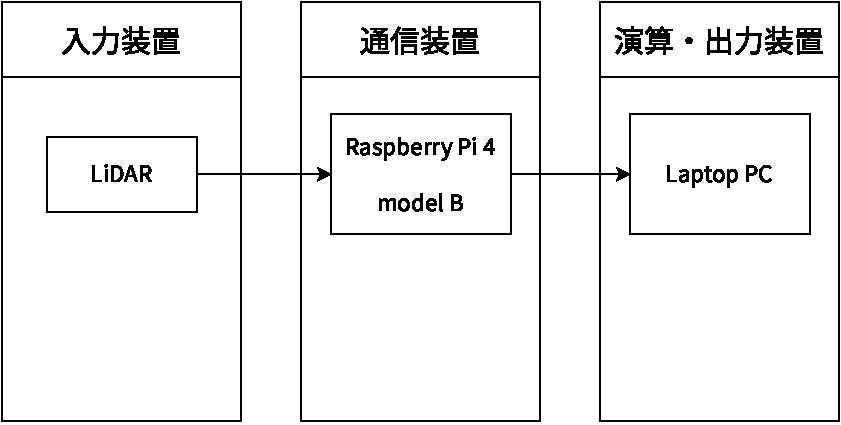
\includegraphics[width=.6\linewidth]{img/slam_21.pdf}
  \caption{環境地図作成システムの概要}
  \label{slam:hard}
  \end{center}
\end{figure}

通信装置では、Raspberry Pi がROSシステム上のマスターノードとして機能してスレーブノードであるLaptop PCと通信を行う。
演算・出力装置では、Laptop PCがマッピングの処理を行う。
ROSのシステムをマスターとスレーブに分割することで、分散処理により、マッピング等の演算機能をRaspberry Piよりも処理速度が速いノートPCで行うことができる。
また、通信装置に使用しているRaspberry Piは、将来的に自律移動ロボットに組み込むことを想定し、
アクチュエータ制御を担うArduinoとの通信を行うことも目的としており、ROSの通信機能によって自律移動の情報をLaptopとArduinoに送受信する。
Raspberry Piに接続したLiDARの点群取得の実行ファイルを以下に示す。LiDARは、北陽電機社製のURG-04LX-UG01を用いた。
ROS上で北陽電機社製のLiDARを扱うためのドライバとしてurg\verb|_|node\cite{slam:urg}を用いる。
LiDARによる点群取得の実行ファイルをソースコード\ref{slam:s1}に示す。

\begin{lrbox}{\mybox}
  \begin{lstlisting}[caption=LiDARによる点群取得の実行ファイル,label=slam:s1]
<launch>
  <node pkg="urg_node" name="urg_node" type="urg_node" output="screen" >
    <param name="serial_port" value="/dev/ttyACM0"/>
    <param name="serial_baud" value="115200"/>
    <param name="frame_id" value="base_link"/>
    <param name="calibrate_time" value="true"/>
    <param name="publish_intensity" value="false"/>
    <param name="publish_multiecho" value="false"/>
    <param name="angle_min" value="-1.5707963"/>
    <param name="angle_max" value="1.5707963"/>
  </node>
</launch>
  \end{lstlisting}
\end{lrbox}
\scalebox{.9}{\usebox{\mybox}}

\subsubsection{ソフトウェア}
LiDARのスキャンによって得られるランドマークの位置情報を、自己位置を示すロボット座標系と、地図の座標系に変換する。
座標変換はROSのtf\cite{slam:tf}パッケージを用いて行い、それぞれのSLAMアルゴリズムの実装に合わせて必要な座標系を取得するように実装する。

次にそれぞれのSLAMアルゴリズムにおいて、地図作成に使用した座標系の取り扱いの違いについて説明する。

\subsubsection{Gmapping,Cartographer}
GmappingとCartographerに関しては、LiDARのスキャンをロボット座標系に変換し、
laser\verb|_|scan\verb|_|matcher\cite{slam:laser}パッケージを用いて
オドメトリとマッチングさせることで、地図を作成する。それぞれの座標変換の概要tfツリーを図\ref{slam:tf1}、\ref{slam:tf2}に示す。

\begin{figure}[h]
  \begin{center}
  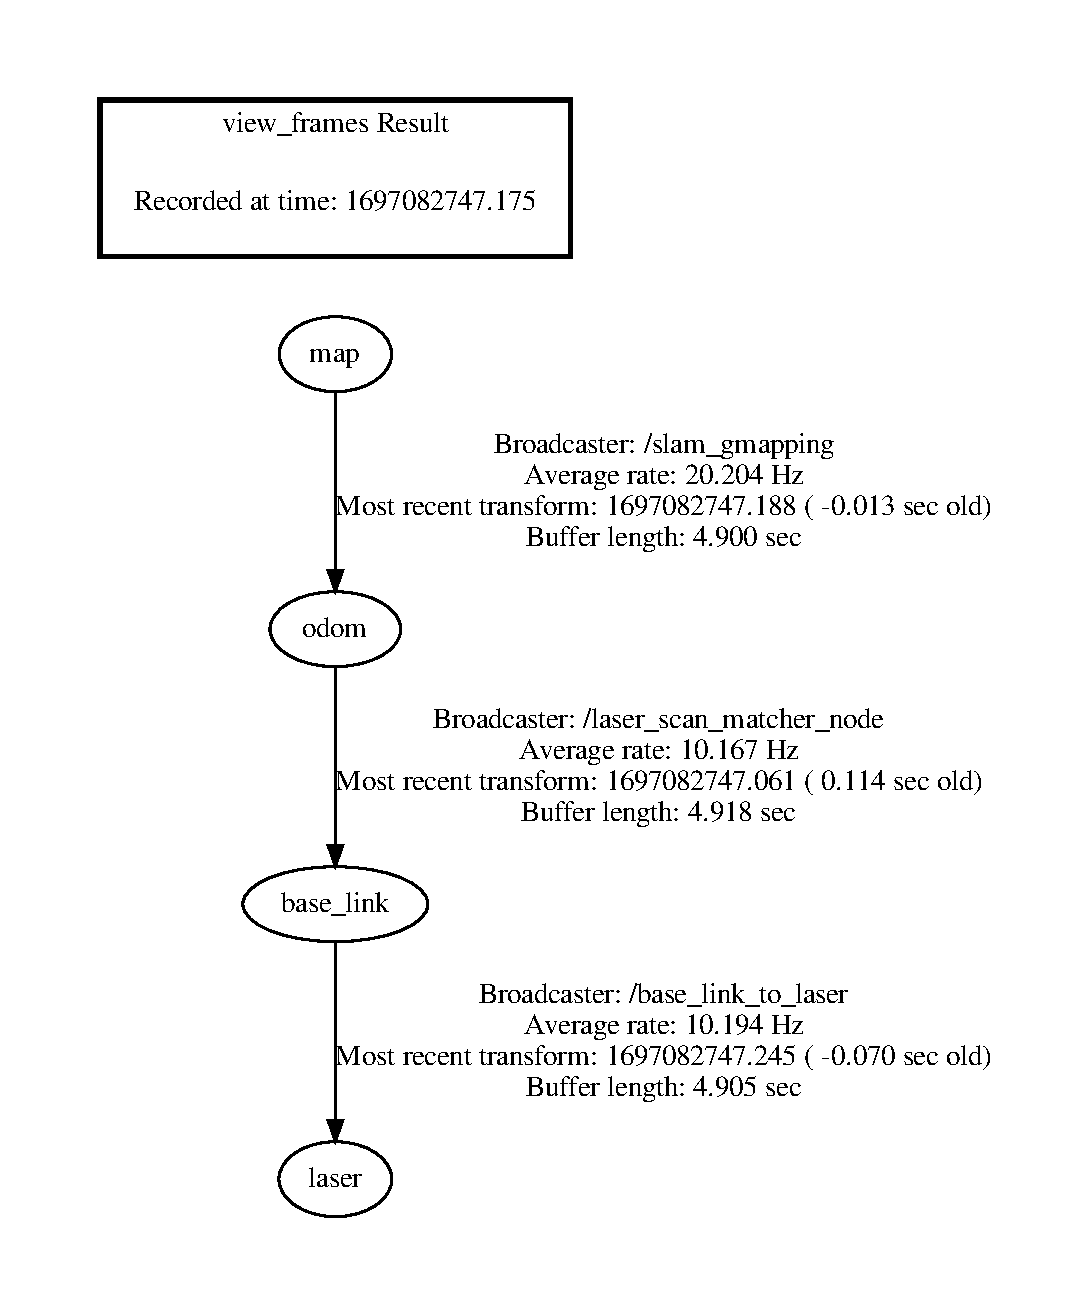
\includegraphics[width=.8\linewidth]{img/slam_22.pdf}
  \caption{Gmappingの座標変換tfツリー}
  \label{slam:tf1}
  \end{center}
\end{figure}

\begin{figure}[h]
  \begin{center}
  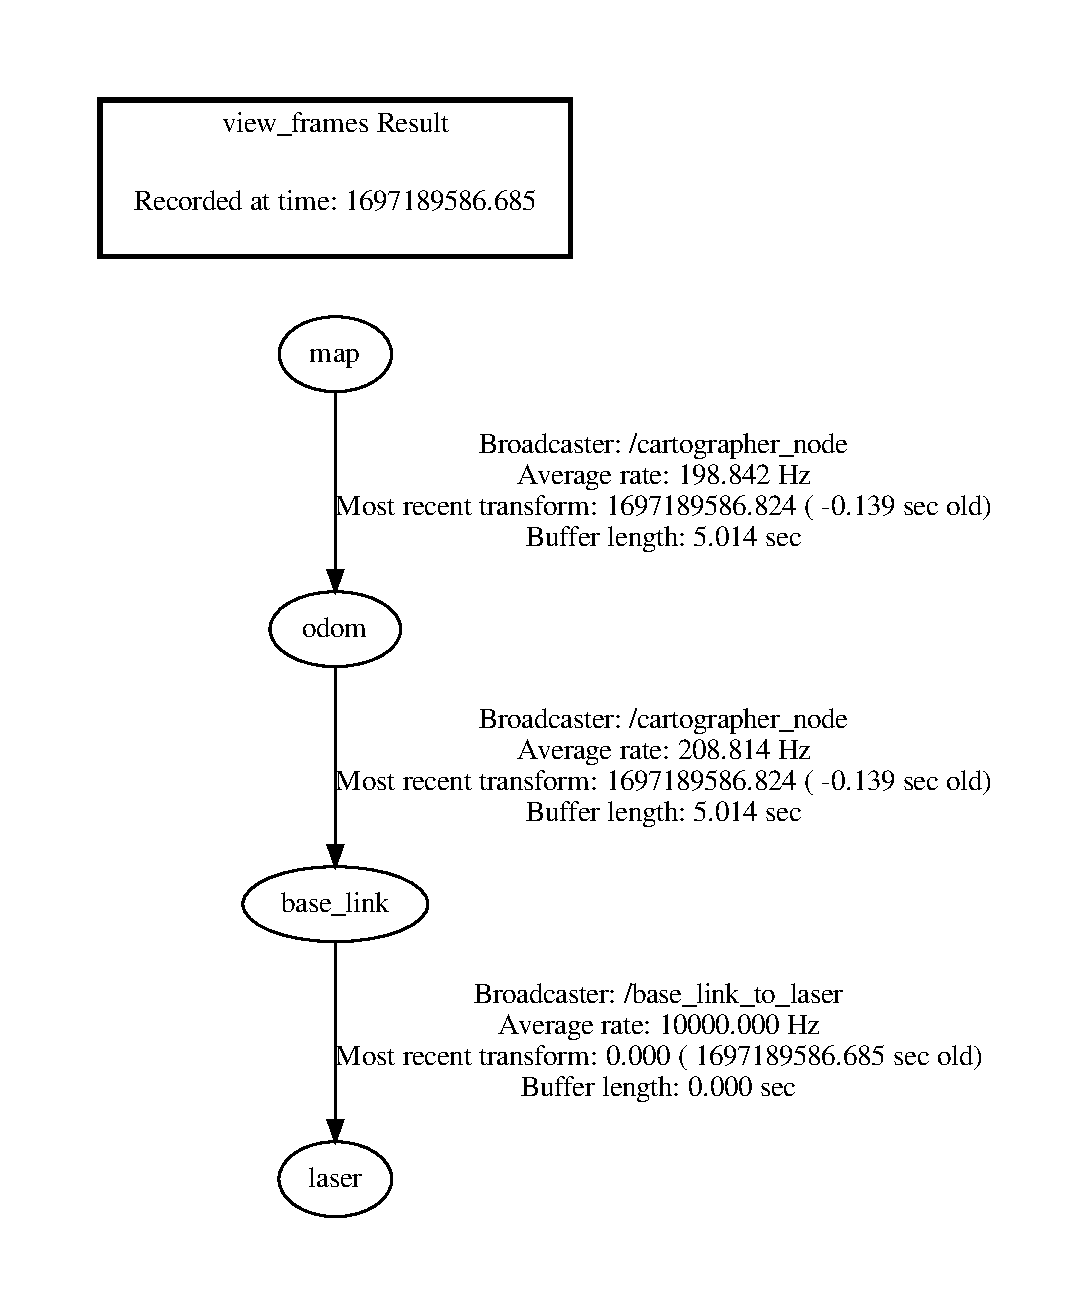
\includegraphics[width=.8\linewidth]{img/slam_23.pdf}
  \caption{Cartographerの座標変換tfツリー}
  \label{slam:tf2}
  \end{center}
\end{figure}

\clearpage

\subsubsection{laser scan matcher}
laser\verb|_|scan\verb|_|matcherは、2つの点群に関して、その位置関係を推定して合成することを行うROSのパッケージであり、
レーザスキャンの移動の増分を取得する機能を有する。このパッケージでは、\verb|sensor_msgs/LaserScan|メッセージ間のスキャンマッチングを可能にし、レーザの推定位置を\verb|geometry_msgs/Pose2D|またはtfのメッセージとして取得する。
このパッケージは、LiDAR以外のセンサによって得られるオドメトリ無しで使用することができる。また、複数の種類のオドメトリを追加することで、
LiDAR自身のレーザスキャンの取得速度と精度を向上させることができる。

\subsubsection{laser scan matcherの原理}
laser\verb|_|scan\verb|_|matcherは、点群のスキャンマッチングとして有名なICPアルゴリズム\cite{slam:icp}の派生版であるPLICP(Point to Line ICP)\cite{slam:plicp}が実装されている。

まず、ICPアルゴリズム(Iterative Closest Point)について述べる。ICPアルゴリズムでは、2つの点群が整合するように、その位置姿勢の関係を調整する方法の1つである。ICPでは、
図\ref{slam:icp1}に示す。ように繰り返し計算に基づいて、段階的に位置姿勢を調整する。

\begin{figure}[h]
  \begin{center}
    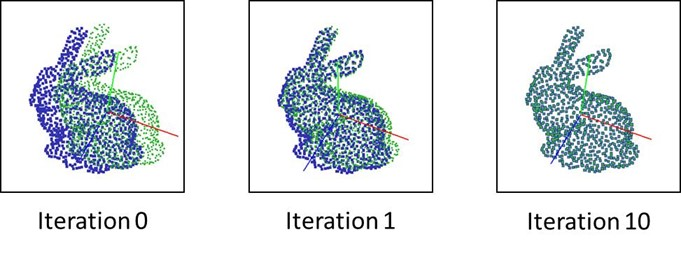
\includegraphics[width=.8\linewidth]{img/slam_24.jpg}
    \caption{ICPアルゴリズムの繰り返しの様子}
    \label{slam:icp1}
  \end{center}
\end{figure}

次にICPの処理の手順を説明する。ICPのアルゴリズムの繰り返しの様子を図\ref{slam:icp_process}に示す。
\begin{enumerate}
  \item 片側の点群Aの各点から、もう片方の点群Bで最近傍の点を探索し、対応づける。
  \item 対応づけた点の差を最小化するように、点群の座標系の位置姿勢を調整する。
\end{enumerate}

処理1の時点で2つの点群のずれが大きいと、対応付けは間違いを含みやすくなる。この場合、処理2の調整結果は
ずれが残る場合がある。そこで、繰り返し計算による精度向上を考える。まず処理2の後、2つの点群のずれは初期の状態より小さくなっていると仮定する。
その状態で再度処理1を行えば、初期の状態より正確に対応付けができることが期待できる。そして、対応付けが正確にできれば処理2の位置姿勢も正確に調整できる。
つまり、繰り返し計算を行うことで、徐々に精度を向上させることができる。

\begin{figure}[h]
  \begin{center}
    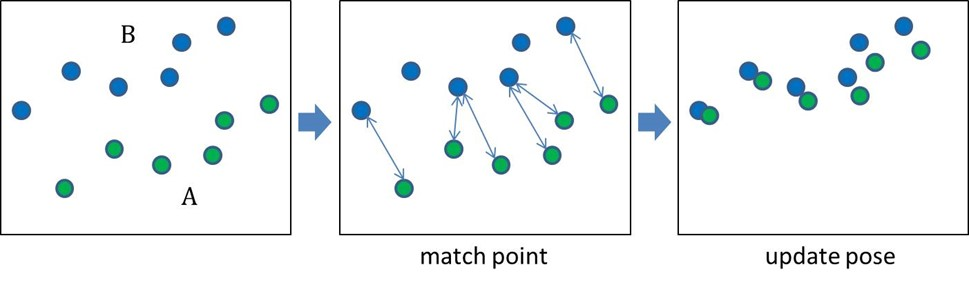
\includegraphics[width=.8\linewidth]{img/slam_25.jpg}
    \caption{ICPアルゴリズムの繰り返しの様子}
    \label{slam:icp_process}
  \end{center}
\end{figure}

ICP方式には次のような欠点がある。
\begin{enumerate}
  \item 初期値に依存し、初期値が悪いと反復回数が増加し、初期誤差が大きい場合は、反復結果を誤ることがある。
  \item ICPは一次収束であり、収束速度が遅い。(探索効率を上げるためにkd-treeを使うことになる。)
  \item 異常値やノイズが発生する。
\end{enumerate}

PLICPは、ICPアルゴリズムを改良し、標準の点と点のマッチングではなく、点と線のマッチングを行う。PLICPを図\ref{slam:plicp}に示す。
PLICPの処理は、ICPと同じである。違いは、ICPが最近傍点を見つけて点間の距離を誤差として使用するのに対し、PLICPは2つの最近傍点を見つけることである。2つの点を接続する場合、
点から線までの距離が誤差として使用されるため、PLICPのマッチングエラーはICPのマッチングエラーよりもはるかに小さくなる。

\begin{figure}[h]
  \begin{center}
    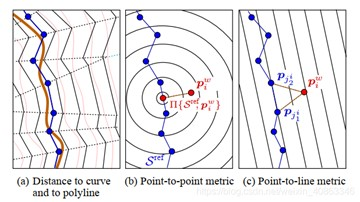
\includegraphics[width=.8\linewidth]{img/slam_26.jpg}
    \caption{PLICP\cite{slam:plicp}}
    \label{slam:plicp}
  \end{center}
\end{figure}

図\ref{slam:plicp_p1p2}にPLICPによるP1とP2の位置関係を示す。
青い点は$t-1$時間のレーザ点、茶色の線(壁など)、赤い点は時点実際のオブジェクト図中の同心円の実践は点間の距離誤差を表す。点P1を知るある点からの距離Dによって別の点P2の位置が決まる。P2の位置は、P1を中心とし、
Dを半径とする円上にある。

\begin{figure}[h]
  \begin{center}
    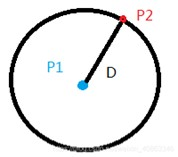
\includegraphics[width=.3\linewidth]{img/slam_27.jpg}
    \caption{PLICPによるP1とP2の位置関係\cite{slam:china}}
    \label{slam:plicp_p1p2}
  \end{center}
\end{figure}

文献\cite{slam:china}によると、PLICPがICP、IDC、MBICP等のアルゴリズムよりも精度が高く、反復回数が少なくて済むことが示されている。
また、アルゴリズムの最適化技術により、PLICPは高速に動作することが述べられている。

\subsubsection{Hector SLAM}
図\ref{slam:tf3}にHector SLAMの座標変換のtfツリーを示す。Hector SLAMに関しては、LiDARのスキャンをロボットの座標系に変換した後に、ロボット座標系の移動履歴の座標系をtfのみでオドメトリを生成し、
ロボット座標系に変換する前のLiDARのスキャンとマッチングさせることで、地図を作成する。

\begin{figure}[h]
  \begin{center}
  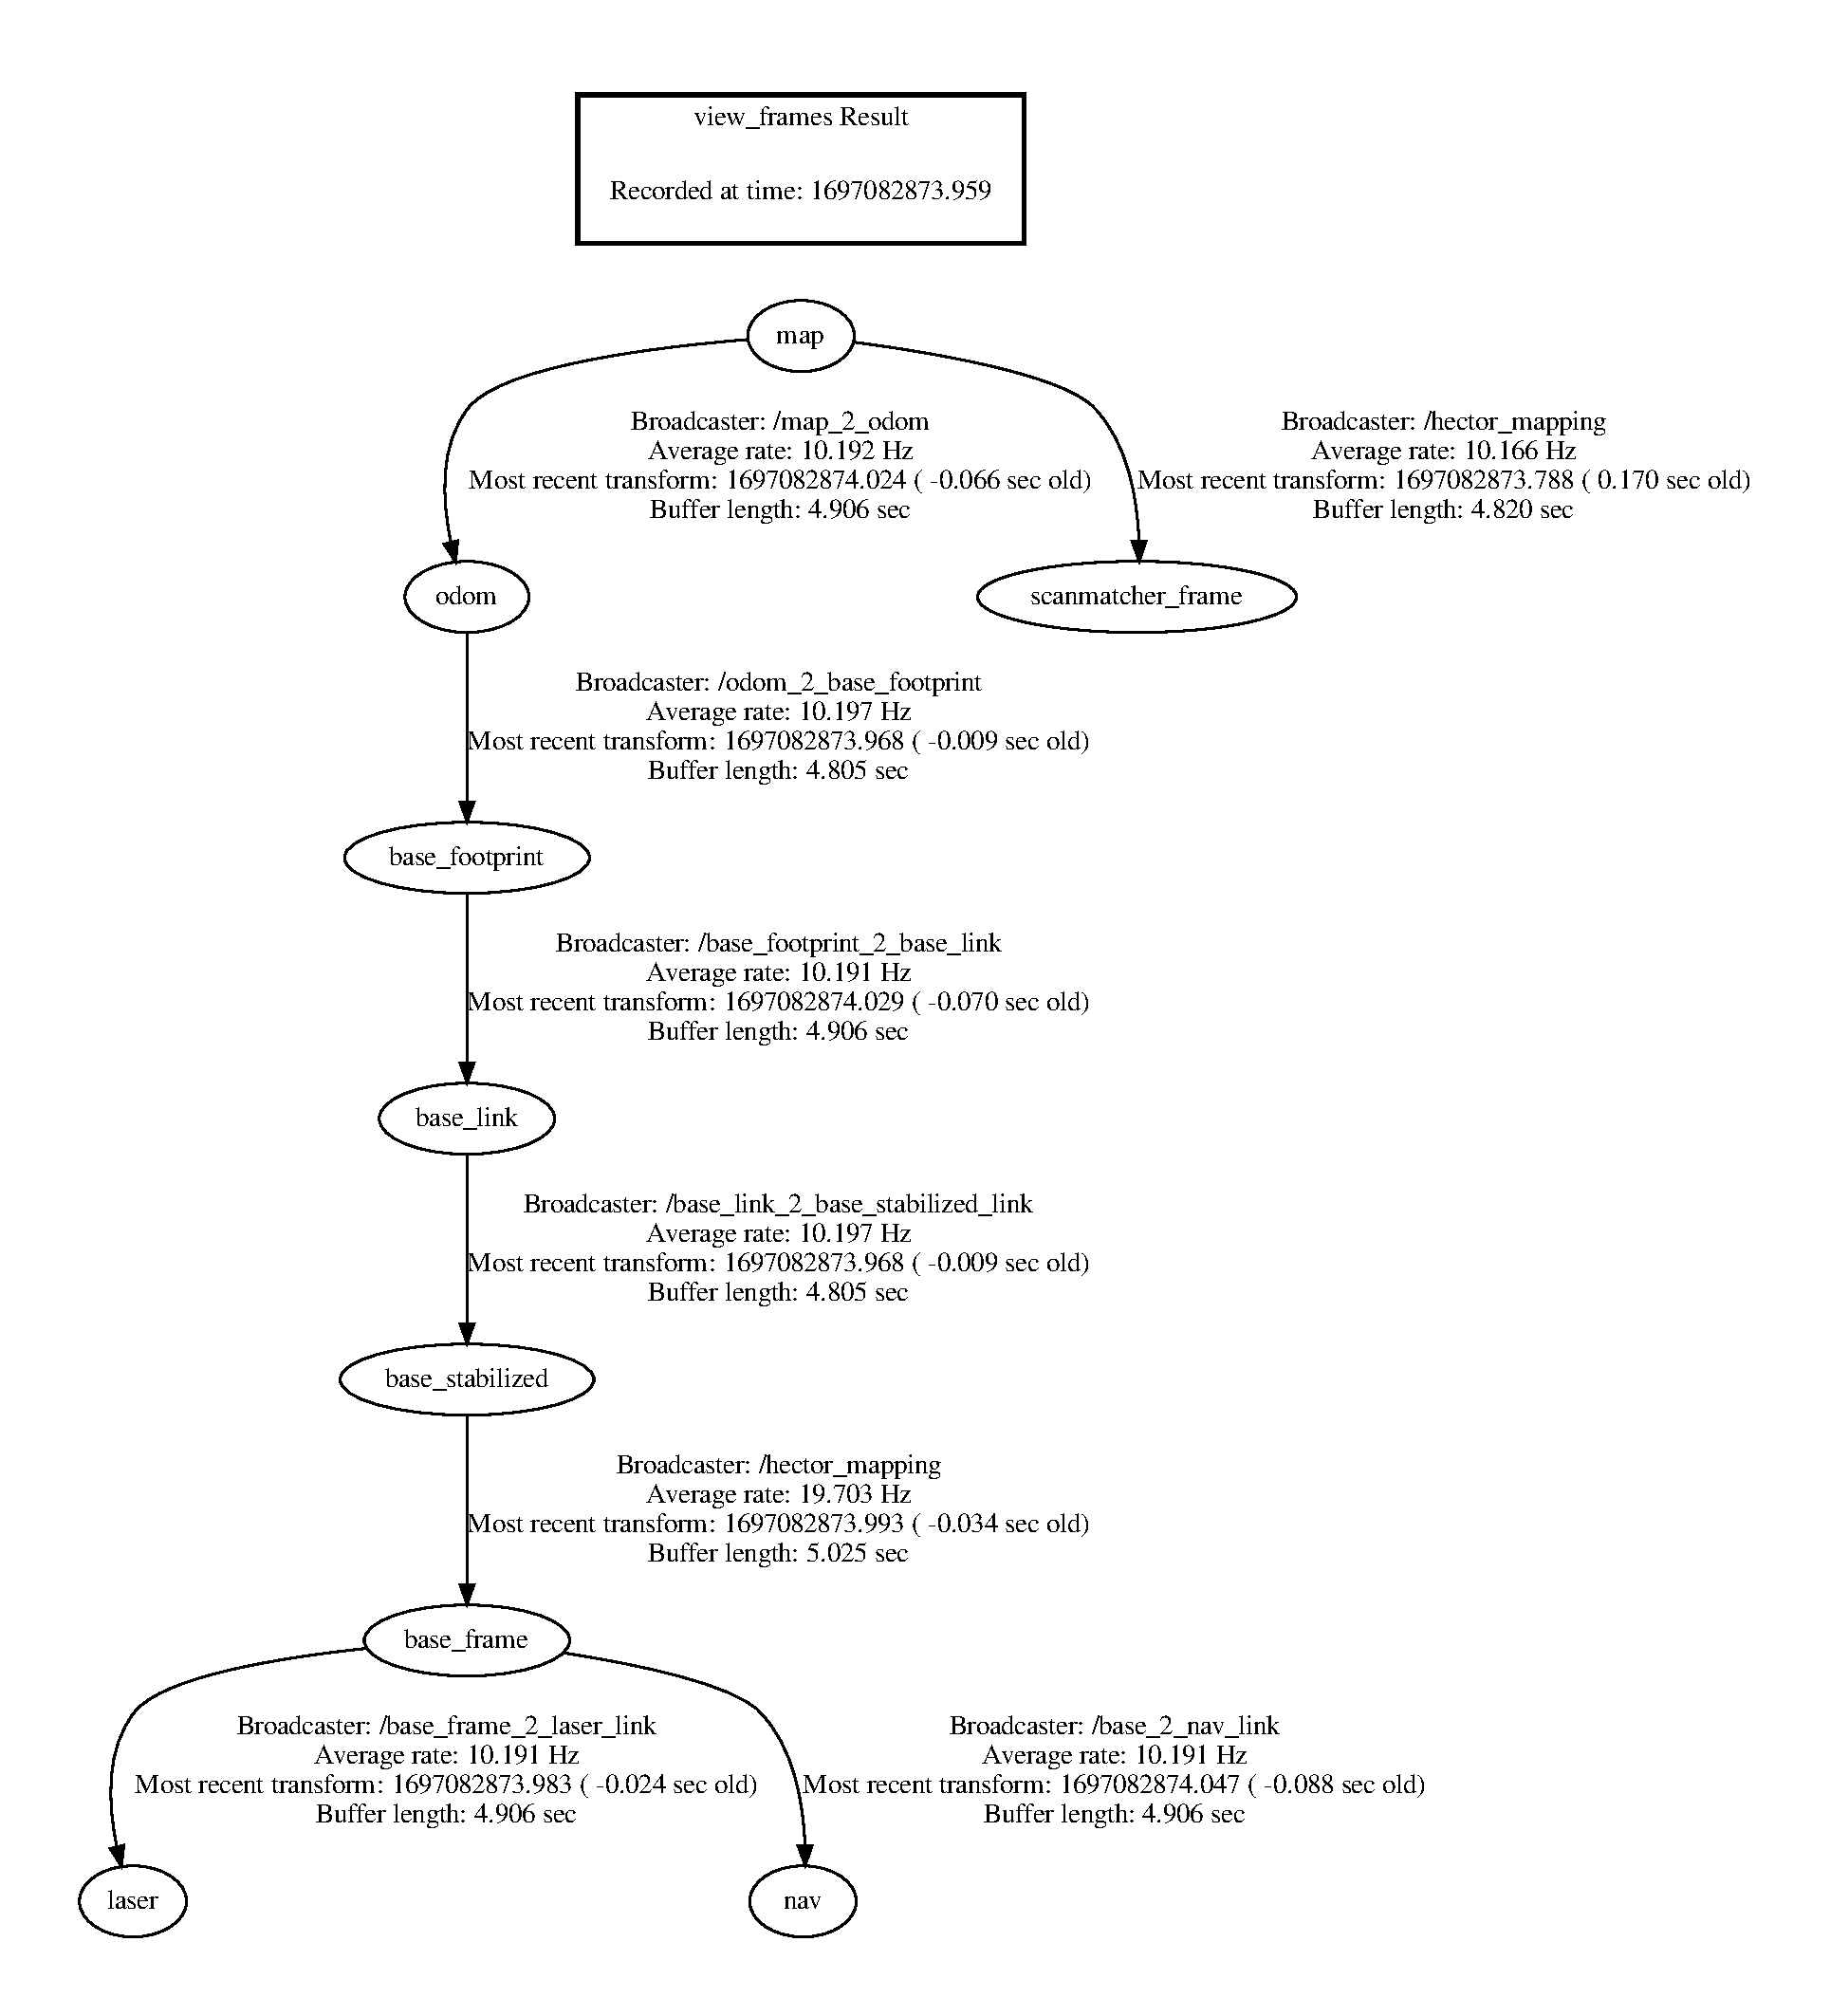
\includegraphics[width=.8\linewidth]{img/slam_28.pdf}
  \caption{Hector SLAMの座標変換tfツリー}
  \label{slam:tf3}
  \end{center}
\end{figure}

\clearpage

\subsubsection{パラメータの調整}
各SLAMパッケージのパラメータの値を示す。

\begin{lrbox}{\mybox}
\begin{lstlisting}[caption=Gmappingのレーザオドメトリのパラメータ,label=slam:s2]
<?xml version="1.0"?>
<launch>
  <node pkg="tf" type="static_transform_publisher" name="base_link_to_laser" args="0.0 0 0 0.0 0.0 0.0 /base_link /laser 100" />
//LiDARスキャン(laser)をロボット座標(base_link)に変換
  <node pkg="laser_scan_matcher" type="laser_scan_matcher_node" name="laser_scan_matcher_node">
    <param name="fixed_frame" value = "/odom"/>//地図座標
    <param name="base_frame" value = "/base_link"/>//ロボット座標
    <param name="use_cloud_input" value="false"/>
    <param name="publish_tf" value="true"/>
    <param name="publish_odom" value="true"/>
    <param name="use_odom" value="false"/>
    <param name="use_imu" value="false"/>
    <param name="use_alpha_beta" value="true"/>
    <param name="max_iterations" value="10"/>
  </node>
</launch>
\end{lstlisting}
\end{lrbox}
\scalebox{.9}{\usebox{\mybox}}

\begin{lrbox}{\mybox}
\begin{lstlisting}[caption=Gmappingの座標系の設定,label=slam:s3]
<launch>
  <node pkg="gmapping" type="slam_gmapping" name="slam_gmapping" clear_params="true">
    <rosparam command="load" file="$(find urg_gmapping)/config/gmapping.yaml" />
    <!-- <remap from="scan" to="front_laser/scan" /> -->
    <param name="base_frame" value="/base_link" />
    <param name="odom_frame" value="/odom" />
    <param name="map_frame"  value="/map" />
  </node>
  <node pkg="rviz" type="rviz" name="rviz" args="-d $(find urg_gmapping)/rviz_cfg/rviz_cfg.rviz"/>
</launch>
\end{lstlisting}
\end{lrbox}
\scalebox{.9}{\usebox{\mybox}}

\begin{lrbox}{\mybox}
\begin{lstlisting}[caption=Hector SLAMの座標系の設定,label=slam:s4]
<?xml version="1.0"?>
<launch>
  <arg name="tf_map_scanmatch_transform_frame_name" default="scanmatcher_frame"/>
  <arg name="base_frame" default="base_footprint"/>
  <arg name="odom_frame" default="nav"/>
  <arg name="pub_map_odom_transform" default="true"/>
  <arg name="scan_subscriber_queue_size" default="5"/>
  <arg name="scan_topic" default="scan"/>
  <arg name="map_size" default="2048"/>
  
  <node pkg="hector_mapping" type="hector_mapping" name="hector_mapping" output="screen">
    
    <!-- Frame names -->
    <param name="map_frame" value="map" />
    <param name="base_frame" value="$(arg base_frame)" />
    <param name="odom_frame" value="$(arg odom_frame)" />
    
    <!-- Tf use -->
    <param name="use_tf_scan_transformation" value="true"/>
    <param name="use_tf_pose_start_estimate" value="false"/>
    <param name="pub_map_odom_transform" value="$(arg pub_map_odom_transform)"/>
    
    <!-- Map size / start point -->
    <param name="map_resolution" value="0.050"/>
    <param name="map_size" value="$(arg map_size)"/>
    <param name="map_start_x" value="0.5"/>
    <param name="map_start_y" value="0.5" />
    <param name="map_multi_res_levels" value="2" />
    
    <!-- Map update parameters -->
    <param name="update_factor_free" value="0.4"/>
    <param name="update_factor_occupied" value="0.9" />    
    <param name="map_update_distance_thresh" value="0.4"/>
    <param name="map_update_angle_thresh" value="0.06" />
    <param name="laser_z_min_value" value = "-1.0" />
    <param name="laser_z_max_value" value = "1.0" />
    
    <!-- Advertising config --> 
    <param name="advertise_map_service" value="true"/>
    
    <param name="scan_subscriber_queue_size" value="$(arg scan_subscriber_queue_size)"/>
    <param name="scan_topic" value="$(arg scan_topic)"/>
    
    <param name="tf_map_scanmatch_transform_frame_name" value="$(arg tf_map_scanmatch_transform_frame_name)" />
  </node>
  <node pkg="tf" type="static_transform_publisher" name="map_2_odom" args="0 0 0 0 0 0 /map /odom 100"/>
  <node pkg="tf" type="static_transform_publisher" name="odom_2_base_footprint" args="0 0 0 0 0 0 /odom /base_footprint 100"/>
  <node pkg="tf" type="static_transform_publisher" name="base_footprint_2_base_link" args="0 0 0 0 0 0 /base_footprint /base_link 100"/> 
  <node pkg="tf" type="static_transform_publisher" name="base_link_2_base_stabilized_link" args="0 0 0 0 0 0 /base_link /base_stabilized 100"/> 
  <node pkg="tf" type="static_transform_publisher" name="base_stablized_2_base_frame" args="0 0 0 0 0 0 /base_stabilized /base_frame 100"/> 
  <node pkg="tf" type="static_transform_publisher" name="base_frame_2_laser_link" args="0 0 0 0 0 0 /base_frame /laser 100"/> 
  <node pkg="tf" type="static_transform_publisher" name="base_2_nav_link" args="0 0 0 0 0 0 /base_frame /nav 100"/>
</launch>
\end{lstlisting}
\end{lrbox}

\begin{lrbox}{\mybox}
\begin{lstlisting}[caption=Cartographerの座標系とレーザオドメトリのパラメータの設定,label=slam:s5]
include "map_builder.lua"
include "trajectory_builder.lua"

options = {
  map_builder = MAP_BUILDER、
  trajectory_builder = TRAJECTORY_BUILDER、
  map_frame = "map"、
  tracking_frame = "base_link"、
  published_frame = "base_link"、
  odom_frame = "odom"、
  provide_odom_frame = true、
  publish_frame_projected_to_2d = true、
  use_odometry = false、
  use_nav_sat = false、
  use_landmarks = false、
  num_laser_scans = 1、
  num_multi_echo_laser_scans = 0、
  num_subdivisions_per_laser_scan = 1、
  num_point_clouds = 0、
  lookup_transform_timeout_sec = 0.2、
  submap_publish_period_sec = 0.3、
  pose_publish_period_sec = 5e-3、
  trajectory_publish_period_sec = 30e-3、
  rangefinder_sampling_ratio = 1.、
  odometry_sampling_ratio = 1.、
  fixed_frame_pose_sampling_ratio = 1.、
  imu_sampling_ratio = 1.、
  landmarks_sampling_ratio = 1.、
}

MAP_BUILDER.use_trajectory_builder_2d = true

TRAJECTORY_BUILDER_2D.min_range = 0.5
TRAJECTORY_BUILDER_2D.max_range = 8.
TRAJECTORY_BUILDER_2D.missing_data_ray_length = 8.5
TRAJECTORY_BUILDER_2D.use_imu_data = false
TRAJECTORY_BUILDER_2D.use_online_correlative_scan_matching = true
TRAJECTORY_BUILDER_2D.real_time_correlative_scan_matcher.linear_search_window = 0.1
TRAJECTORY_BUILDER_2D.real_time_correlative_scan_matcher.translation_delta_cost_weight = 10.
TRAJECTORY_BUILDER_2D.real_time_correlative_scan_matcher.rotation_delta_cost_weight = 1e-1
TRAJECTORY_BUILDER_2D.motion_filter.max_angle_radians = math.rad(0.2)
-- for current lidar only 1 is good value
TRAJECTORY_BUILDER_2D.num_accumulated_range_data = 1

POSE_GRAPH.constraint_builder.min_score = 0.65
POSE_GRAPH.constraint_builder.global_localization_min_score = 0.65
POSE_GRAPH.optimization_problem.huber_scale = 1e2
POSE_GRAPH.optimize_every_n_nodes = 35

return options  
\end{lstlisting}
\end{lrbox}
\scalebox{.9}{\usebox{\mybox}}

\subsubsection{RVizによる環境地図の可視化}
RVizアプリケーション上でロボットプロトタイプが生成する環境地図の可視化のプロセスについて述べる。
SLAMのプログラムによって作成された環境地図は、ROSツールであるmap\verb|_|server によって、pgmとyamlの形式で保存される。
Rvizアプリケーションでこれらの形式を読み込むことができる。Rvizアプリケーションでは、読み込んだ地図の測定ツールがある。
この機能は2点間の距離を計算することができる機能である。計算したい2つの値を取得することで、測定結果をメートル単位で表示する。
図\ref{slam:map:read}にLiDARのスキャン結果を示す。図\ref{slam:map}に環境地図の読み込み画面を示す。
urg\verb|_|nodeでLiDARのscanトピックを生成し、SLAMプログラムがスキャンデータの変換にtfパッケージを使用して、自己位置と地図の演算を行う。
Rvizアプリケーションはマッピングの結果をリアルタイムで表示する。

\begin{figure}[h]
  \begin{center}
  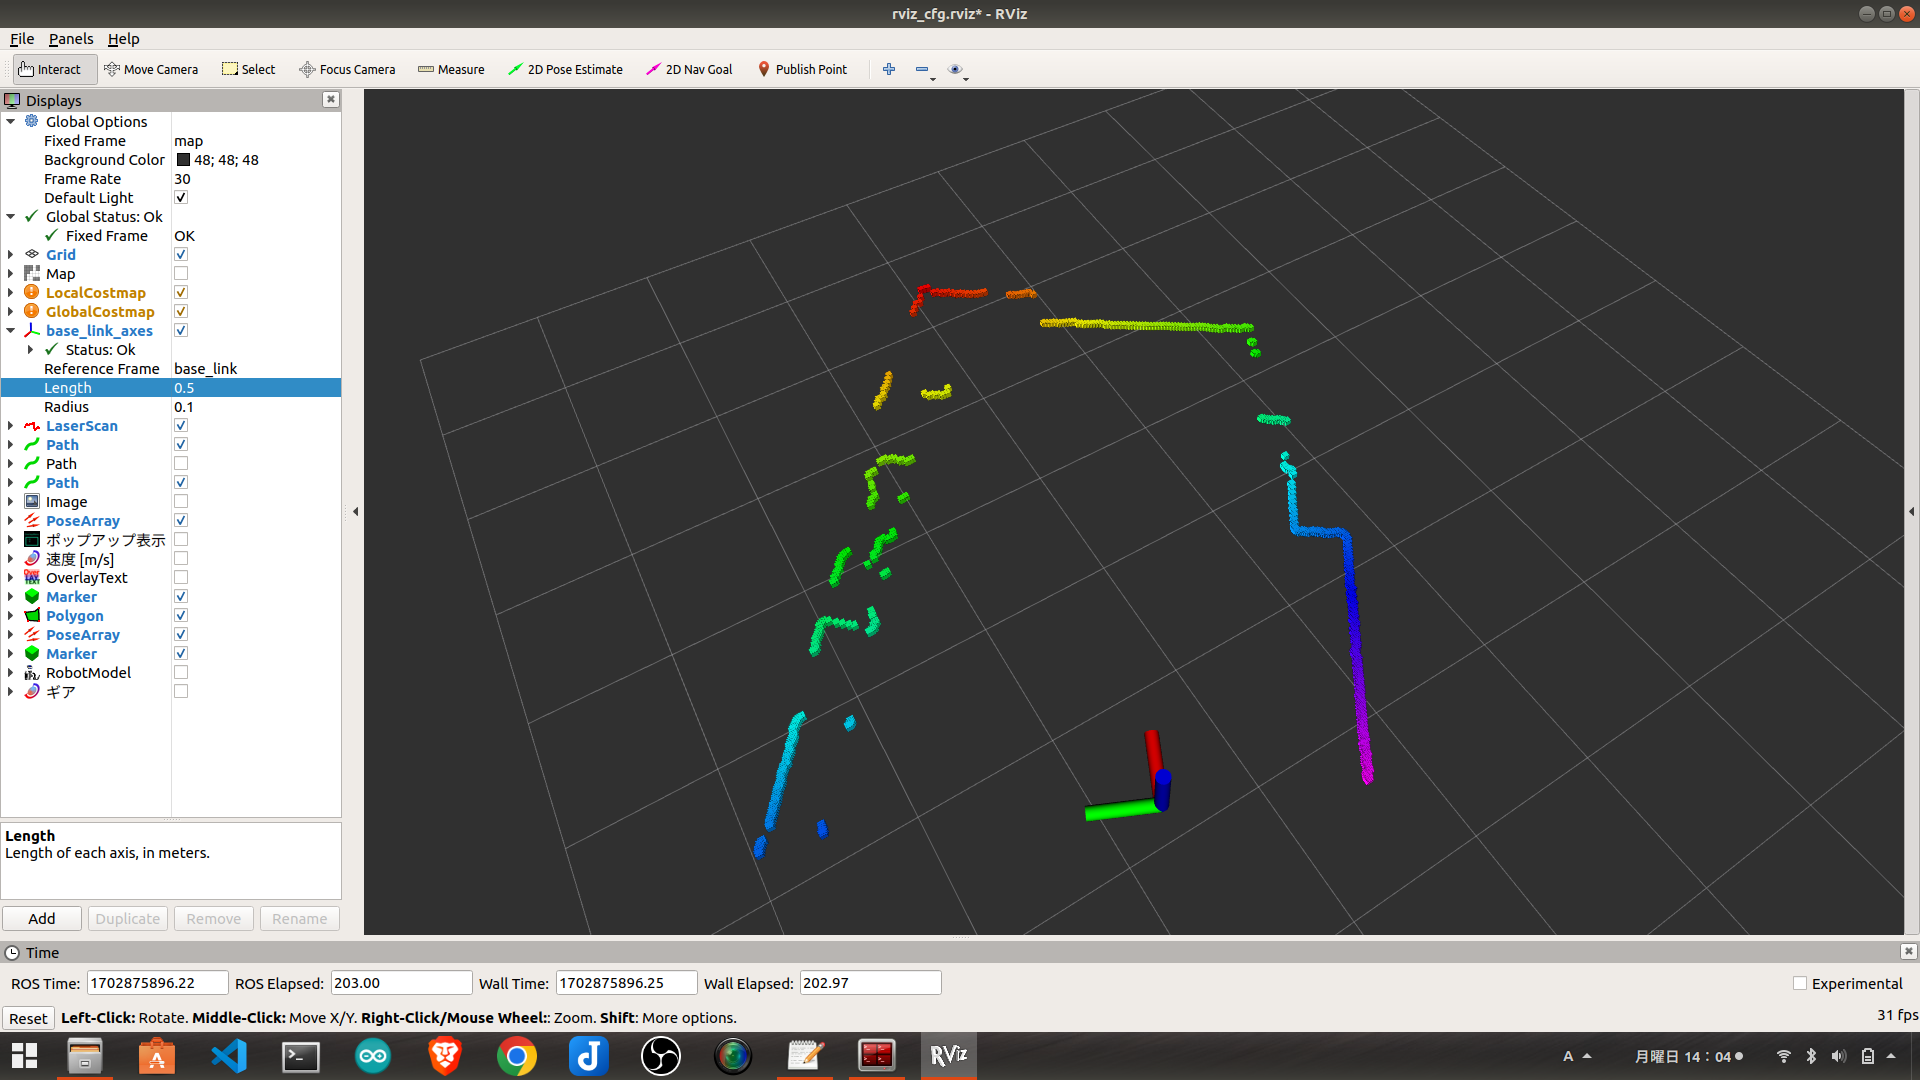
\includegraphics[width=.8\linewidth]{img/slam_29.png}
  \caption{LiDARのスキャン結果}
  \label{slam:map:read}
  \end{center}
\end{figure}

\begin{figure}[h]
  \begin{center}
  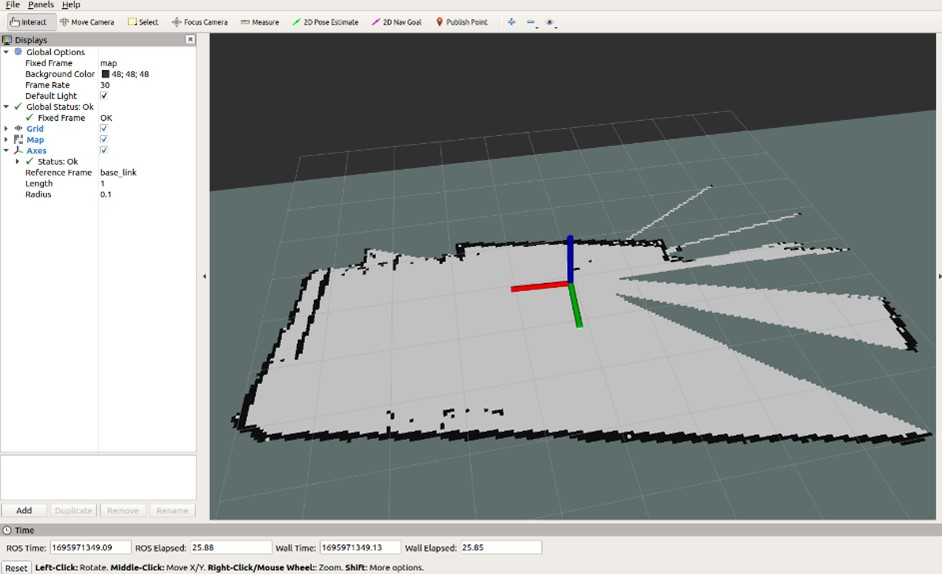
\includegraphics[width=.6\linewidth]{img/slam_30.jpg}
  \caption{環境地図の読み込み}
  \label{slam:map}
  \end{center}
\end{figure}

\section{検証}

\subsection{実験}
本研究で提案した環境地図作成システムを用いて、Gmapping、Hector SLAM、CartographerのSLAMアルゴリズムパッケージを用いて、屋内の一室を用いた環境地図の作成実験を実施した。
今回の屋内環境は一つの部屋のみであり、仕切りなどは存在せず、部屋の基礎部分となる支柱が特徴点として検出しやすいため、SLAMの環境に適している。
部屋の詳細は、図\ref{slam:map:measure}の平面図に示している。
平面図には、部屋の設計寸法から値を使用している。
図\ref{slam:map:place}は、環境地図中の辺に番号を付けたものである。
本実験では、Gmapping、Hector SLAM、Cartographerのアルゴリズムによって生成された環境地図の寸法と実際の寸法との対応の誤差を評価する。
方法としてRviz測定ツールによる手動測定値と実際の寸法の値を比較する。
人が部屋の中でLiDARからなるシステムを持って歩くことで地図を作成する。この際、LiDARの方向を変える際は、ゆっくり行い、人が歩く動作をなるべく慎重に行った。
\begin{figure}[h]
  \begin{center}
  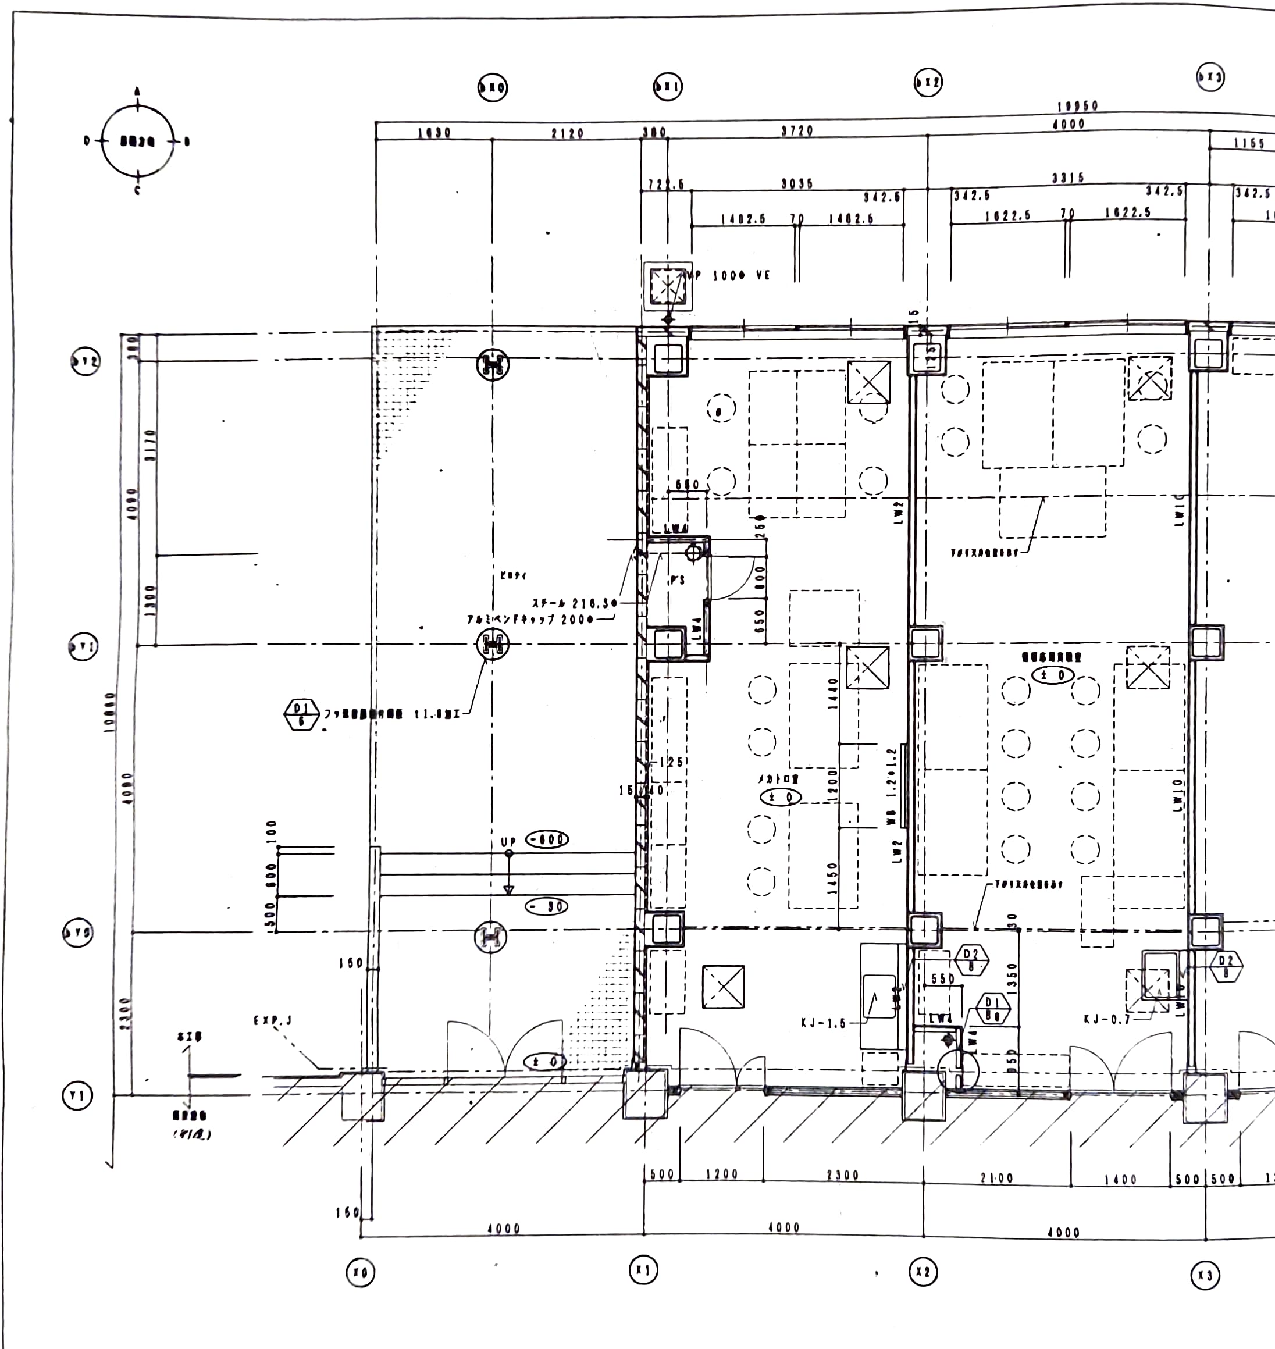
\includegraphics[width=.8\linewidth]{img/slam_31.pdf}
  \caption{実際の部屋の寸法図}
  \label{slam:map:measure}
  \end{center}
\end{figure}

\begin{figure}[h]
  \begin{center}
  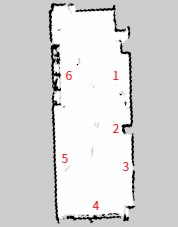
\includegraphics[width=.8\linewidth]{img/slam_32.jpg}
  \caption{寸法の測定箇所}
  \label{slam:map:place}
  \end{center}
\end{figure}

\clearpage

\subsection{結果}
Gmapping、Hector SLAM、CartographerともにRVizの画面上に環境地図が描画された。
図\ref{slam:map:gmapping}\verb|~|\ref{slam:map:cartographer}に各アルゴリズムによって生成された環境地図を示す。
内界センサによるオドメトリを用いず、LiDARのみでSLAMを行っているが、部屋の特徴を的確にとらえており、実際の部屋と同様に支柱の構造
と収納棚が確認され、非対称な形状が環境地図に反映されていることが分かる。平面地図の計測の結果を表\ref{slam:table4}に示す。

\begin{figure}[h]
  \begin{center}
  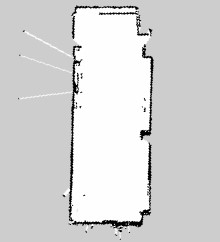
\includegraphics[width=.8\linewidth]{img/slam_33.jpg}
  \caption{Gmapping}
  \label{slam:map:gmapping}
  \end{center}
\end{figure}

\begin{figure}[h]
  \begin{center}
  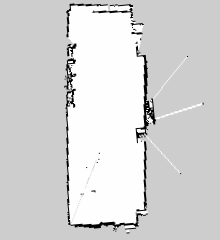
\includegraphics[width=.8\linewidth]{img/slam_34.png}
  \caption{HectorSLAM}
  \label{slam:map:hectorslam}
  \end{center}
\end{figure}

\begin{figure}[h]
  \begin{center}
  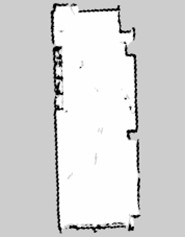
\includegraphics[width=.8\linewidth]{img/slam_35.jpg}
  \caption{Cartographer}
  \label{slam:map:cartographer}
  \end{center}
\end{figure}

\begin{table}[h]
  \centering
  \caption{RVizの測定ツールによる測定結果}
  \scalebox{.75}{
  \begin{tabular}{@{}crrrrrrr@{}}
  \toprule
  No                   & \multicolumn{4}{c}{測定値(cm)}                                                                                               & \multicolumn{3}{c}{誤差(cm)}                                                                       \\ \midrule
  \multicolumn{1}{l}{} & \multicolumn{1}{c}{Gmapping} & \multicolumn{1}{c}{HectorSLAM} & \multicolumn{1}{c}{Cartographer} & \multicolumn{1}{c}{実寸} & \multicolumn{1}{c}{Gmapping} & \multicolumn{1}{c}{HectorSLAM} & \multicolumn{1}{c}{Cartographer} \\
  1                    & 361.531                      & 356.567                        & 359.158                          & 356.5                  & 5.031                        & 0.067                          & 2.658                            \\
  2                    & 47.8064                      & 59.3467                        & 51.7346                          & 52.5                   & -4.6936                      & 6.8467                         & -0.7654                          \\
  3                    & 362.027                      & 333.141                        & 359.743                          & 356.5                  & 5.527                        & -23.359                        & 3.243                            \\
  4                    & 338.146                      & 331.471                        & 333.615                          & 331.5                  & 6.646                        & -0.029                         & 2.115                            \\
  5                    & 1067.5                       & 1083.04                        & 1073.81                          & 1074.3                 & 5.845                        & 4.427                          & 3.108                            \\
  6                    & 309.045                      & 307.627                        & 306.308                          & 303.2                  & 5.845                        & 4.427                          & 3.108                            \\
  \multicolumn{5}{c}{平均二乗誤差}  
\label{slam:table4}                                                                                                                     & 5.6051                       & 19.150                         & 0.90262                          \\ \bottomrule
\end{tabular}}
\end{table}

\clearpage

実験番号1、2の実際の寸法が356.5 \si{[cm]}、52.50 \si{[cm]}であることに対して、Gmappingの測定値が361.531 \si{[cm]}、47.8064 \si{[cm]}であったためRviz測定ツールによる測定値と実際の寸法との誤差は5.031 \si{[cm]}、-4.6936 \si{[cm]}となる。
実験番号2 \verb|~|7で示された異なる場所で同様に測定したところ、平均二乗誤差は5.605 \si{[cm]}であった。
このことからlaser\verb|_|scan\verb|_|matcherを使用するGmappingでは5.605 \si{[cm]}の誤差で部屋の地図を作成できることが分かる。
Hector SLAMによって生成された地図の場合、実験番号1、2の測定値が356.567 \si{[cm]}, 59.3467 \si{[cm]}の測定値が得られる。
他も同様に359.743 \si{[cm]}、333.615 \si{[cm]}、1073.81 \si{[cm]}、306.308 \si{[cm]}の結果が得られた。
これらの平均二乗誤差は、19.15 \si{[cm]} であり、Hector SLAMによる地図の寸法にばらつきがあることが分かる。
また、Hector SLAMアルゴリズムを使用した場合、実験番号1の上面と、2の横面、下面に点群のずれが生じている。
Hector SLAMやCartographerは、地図作成の際のLiDARの方向転換や、前進速度等が少しでも早くなると、地図に大きな歪みが生じた。
Hector SLAMは、地図が歪むと修正されない。Cartographerや、Gmappingは、限度があるものの、歪みは修正される。
Gmappingは、地図作成の際のLiDARの方向転換や、前進速度等が速くの影響をほとんど受けなかった。
Cartographerアルゴリズムによって生成された地図の場合、どの実験番号でも誤差が高々3\si{[cm]} 程度であり、
平均二乗誤差が0.90 \si{[cm]} と非常にばらつきが少なく、誤差が少ないことが明らかになった。

\section{考察}
実験の結果より、LiDAR以外の内界センサを用いず、LiDARのみによって地図の生成を行うことが可能であると言える。
特に、平均二乗誤差が最も少ない、Cartographerが他のアルゴリズムと比べて、精度の良い地図であると考えられる。
次点にGmappingの地図の精度が高く、Hector SLAMが最も精度が低い地図となった。
しかし、測定の際の動作を丁寧に行う必要があるアルゴリズムと、測定の際の外乱に強いアルゴリズムが存在することが明らかになった。
今回の実験では、LiDAR計測方向の転換や、歩きながら地図を作成する動作を慎重に実施した、Hector SLAMは、これらの動作を慎重に行わなかった場合、正確な地図を作成することが不可能であった。
これは、LiDARの筐体が移動する速度が速い場合、現在の測定データの端点が、それまでに読み込んで生成した地図のデータ(過去の測定データ)と離れすぎてしまい正しくスキャンマッチングができなくなったためだと考えられる。
また、移動ロボットの現在位置が生成した環境地図から大きくずれてしまい、自己位置を見失う現象が生じた。
その後、復帰することがなかったため、正しいスキャンマッチングができず、別の地形と判断されたためだと考えられる。
Cartographerは、平均二乗誤差が最も少ないが、LiDARの筐体を移動させる速度を速くすることにより、地図が歪む現象が起きた、その後、地図は修正されるが、歪みの分と、元の地図との間の位置へと修正されるが、歪みの量が大きいと、復帰が不可能である。
Gmappingは、移動速度を速くしても、地図の歪みが比較的小さく、現在のスキャンに歪みが含まれても、元の地図の位置とマッチングするように修正が行われる。
これは、他のSLAMアルゴリズムと比べて計算量が少なく、復帰に要する時間が少なかったためだと考えられる。よって、ロボットに搭載して、移動させながら地図を作成する場合、Gmappingを用いることが、妥当であると考えられる。

\clearpage

\section{おわりに}
LiDAR(URG-04LX-01)のみでの地図生成が可能であることを明らかにした。特に、Hector SLAMよりもCartographerやGmappingで生成した地図の精度が 70.7\% ~ 95.3\%
程良いことが明らかになった。また、LiDARによる計測に要する応答性は、Gmappingが、他のアルゴリズムと比べて優れていることが明らかになった。
これらの観点から、比較的、並進速度や角速度が速いロボットの動作において、URG-04LX-01のみで、SLAMを行う場合は、Gmappingを用いることが適切である。
今後は、Gmappingを用いて、4輪自律移動ラジコンカーの開発を行う。